%% Run LaTeX on this file several times to get Table of Contents,
%% cross-references, and citations.

\documentclass[11pt]{book}
\usepackage{gvv}
\usepackage{gvv-book-bkup}
%\usepackage{Wiley-AuthoringTemplate}
\usepackage[sectionbib,authoryear]{natbib}% for name-date citation comment the below line
%\usepackage[sectionbib,numbers]{natbib}% for numbered citation comment the above line

%%********************************************************************%%
%%       How many levels of section head would you like numbered?     %%
%% 0= no section numbers, 1= section, 2= subsection, 3= subsubsection %%
\setcounter{secnumdepth}{3}
%%********************************************************************%%
%%**********************************************************************%%
%%     How many levels of section head would you like to appear in the  %%
%%				Table of Contents?			%%
%% 0= chapter, 1= section, 2= subsection, 3= subsubsection titles.	%%
\setcounter{tocdepth}{2}
%%**********************************************************************%%
\setcounter{tocdepth}{3}
%\includeonly{ch01}
\makeindex

\begin{document}

\frontmatter
%%%%%%%%%%%%%%%%%%%%%%%%%%%%%%%%%%%%%%%%%%%%%%%%%%%%%%%%%%%%%%%%
%% Title Pages
%% Wiley will provide title and copyright page, but you can make
%% your own titlepages if you'd like anyway
%% Setting up title pages, type in the appropriate names here:

\booktitle{CBSE Math}

\subtitle{Made Simple}

\AuAff{G. V. V. Sharma}


%% \\ will start a new line.
%% You may add \affil{} for affiliation, ie,
%\authors{Robert M. Groves\\
%\affil{Universitat de les Illes Balears}
%Floyd J. Fowler, Jr.\\
%\affil{University of New Mexico}
%}

%% Print Half Title and Title Page:
%\halftitlepage
\titlepage

%%%%%%%%%%%%%%%%%%%%%%%%%%%%%%%%%%%%%%%%%%%%%%%%%%%%%%%%%%%%%%%%
%% Copyright Page

\begin{copyrightpage}{2023}
%Title, etc
\end{copyrightpage}

% Note, you must use \ to start indented lines, ie,
% 
% \begin{copyrightpage}{2004}
% Survey Methodology / Robert M. Groves . . . [et al.].
% \       p. cm.---(Wiley series in survey methodology)
% \    ``Wiley-Interscience."
% \    Includes bibliographical references and index.
% \    ISBN 0-471-48348-6 (pbk.)
% \    1. Surveys---Methodology.  2. Social 
% \  sciences---Research---Statistical methods.  I. Groves, Robert M.  II. %
% Series.\\

% HA31.2.S873 2004
% 001.4'33---dc22                                             2004044064
% \end{copyrightpage}

%%%%%%%%%%%%%%%%%%%%%%%%%%%%%%%%%%%%%%%%%%%%%%%%%%%%%%%%%%%%%%%%
%% Only Dedication (optional) 

%\dedication{To my parents}

\tableofcontents

%\listoffigures %optional
%\listoftables  %optional

%% or Contributor Page for edited books
%% before \tableofcontents

%%%%%%%%%%%%%%%%%%%%%%%%%%%%%%%%%%%%%%%%%%%%%%%%%%%%%%%%%%%%%%%%
%  Contributors Page for Edited Book
%%%%%%%%%%%%%%%%%%%%%%%%%%%%%%%%%%%%%%%%%%%%%%%%%%%%%%%%%%%%%%%%

% If your book has chapters written by different authors,
% you'll need a Contributors page.

% Use \begin{contributors}...\end{contributors} and
% then enter each author with the \name{} command, followed
% by the affiliation information.

% \begin{contributors}
% \name{Masayki Abe,} Fujitsu Laboratories Ltd., Fujitsu Limited, Atsugi, Japan
%
% \name{L. A. Akers,} Center for Solid State Electronics Research, Arizona State University, Tempe, Arizona
%
% \name{G. H. Bernstein,} Department of Electrical and Computer Engineering, University of Notre Dame, Notre Dame, South Bend, Indiana; formerly of
% Center for Solid State Electronics Research, Arizona
% State University, Tempe, Arizona 
% \end{contributors}

%%%%%%%%%%%%%%%%%%%%%%%%%%%%%%%%%%%%%%%%%%%%%%%%%%%%%%%%%%%%%%%%
% Optional Foreword:

%\begin{foreword}
%\lipsum[1-2]
%\end{foreword}

%%%%%%%%%%%%%%%%%%%%%%%%%%%%%%%%%%%%%%%%%%%%%%%%%%%%%%%%%%%%%%%%
% Optional Preface:

%\begin{preface}
%\lipsum[1-1]
%\prefaceauthor{}
%\where{place\\
% date}
%\end{preface}

% ie,
% \begin{preface}
% This is an example preface.
% \prefaceauthor{R. K. Watts}
% \where{Durham, North Carolina\\
% September, 2004}

%%%%%%%%%%%%%%%%%%%%%%%%%%%%%%%%%%%%%%%%%%%%%%%%%%%%%%%%%%%%%%%%
% Optional Acknowledgments:

%\acknowledgments
%\lipsum[1-2]
%\authorinitials{I. R. S.}  

%%%%%%%%%%%%%%%%%%%%%%%%%%%%%%%%
%% Glossary Type of Environment:

% \begin{glossary}
% \term{<term>}{<description>}
% \end{glossary}

%%%%%%%%%%%%%%%%%%%%%%%%%%%%%%%%
%\begin{acronyms}
%\acro{ASTA}{Arrivals See Time Averages}
%\acro{BHCA}{Busy Hour Call Attempts}
%\acro{BR}{Bandwidth Reservation}
%\acro{b.u.}{bandwidth unit(s)}
%\acro{CAC}{Call / Connection Admission Control}
%\acro{CBP}{Call Blocking Probability(-ies)}
%\acro{CCS}{Centum Call Seconds}
%\acro{CDTM}{Connection Dependent Threshold Model}
%\acro{CS}{Complete Sharing}
%\acro{DiffServ}{Differentiated Services}
%\acro{EMLM}{Erlang Multirate Loss Model}
%\acro{erl}{The Erlang unit of traffic-load}
%\acro{FIFO}{First in - First out}
%\acro{GB}{Global balance}
%\acro{GoS}{Grade of Service}
%\acro{ICT}{Information and Communication Technology}
%\acro{IntServ}{Integrated Services}
%\acro{IP}{Internet Protocol}
%\acro{ITU-T}{International Telecommunication Unit -- Standardization sector}
%\acro{LB}{Local balance}
%\acro{LHS}{Left hand side}
%\acro{LIFO}{Last in - First out}
%\acro{MMPP}{Markov Modulated Poisson Process}
%\acro{MPLS}{Multiple Protocol Labeling Switching}
%\acro{MRM}{Multi-Retry Model}
%\acro{MTM}{Multi-Threshold Model}
%\acro{PASTA}{Poisson Arrivals See Time Averages}
%\acro{PDF}{Probability Distribution Function}
%\acro{pdf}{probability density function}
%\acro{PFS}{Product Form Solution}
%\acro{QoS}{Quality of Service}
%\acro{r.v.}{random variable(s)}
%\acro{RED}{random early detection}
%\acro{RHS}{Right hand side}
%\acro{RLA}{Reduced Load Approximation}
%\acro{SIRO}{service in random order}
%\acro{SRM}{Single-Retry Model}
%\acro{STM}{Single-Threshold Model}
%\acro{TCP}{Transport Control Protocol}
%\acro{TH}{Threshold(s)}
%\acro{UDP}{User Datagram Protocol}
%\end{acronyms}

\setcounter{page}{1}

\begin{introduction}
This book links high school coordinate geometry to linear algebra and matrix analysis through solved problems.

\end{introduction}

\mainmatter
\chapter{Vectors}
\section{2023}
\subsection{10}
\documentclass{article}
\usepackage{multicol}
\let\vec\mathbf
\begin{document}
\begin{enumerate}
\item In what ratio, does $x$-axis divide the line segment joinin the points $\vec{A}(3,6)$ and $\vec{B}(-12, -3)$ ?
\begin{multicols}{2}
\begin{enumerate}
\item $1:2$
\item $1:4$
\item $4:1$ 
\item $2:1$
\end{enumerate}
\end{multicols}

\item The distance between the point $(0,2\sqrt{5})$ and $(-2\sqrt{5},0)$ is 
\begin{multicols}{2}
\begin{enumerate}
\item $2\sqrt{10}$ units
\item $4\sqrt{10}$ units
\item $2\sqrt{20}$ units
\item $0$ units
\end{enumerate}
\end{multicols}

\item if $(-5,3)$ and $(5,3)$ are two vetices of an equilateral triangle,then coordinates of the third vertex,given that origin lies inside the triangle $(take \sqrt{3}=1.7)$
\item show that the points $(-2,3)$ , $(8,3)$ and $(6,7)$ are the verices of right-angled triangle
\item If $\vec{Q} =(0,1)$ is equidistant from $\vec{P} = (5,-3)$ and $\vec{R} =(x,6)$, find the value of $x$.
\item The distance of the point $(-6,8)$ from origin is :
\begin{multicols}{2}
\begin{enumerate}
\item $6$
\item $-6$
\item $8$
\item $10$
\end{enumerate}
\end{multicols}

\item The points $(-4,0)$ $(4,0)$ and $(0,3)$ are the vertices of $a$ :
\begin{multicols}{2}
\begin{enumerate}
\item right triangle
\item isosceles triangle
\item equilateral triangle
\item scalene triangle
\end{enumerate}
\end{multicols}

\end{enumerate}
\end{document}

\subsection{12}
\begin{enumerate}[label=\thesection.\arabic*.,ref=\thesection.\theenumi]
\numberwithin{equation}{enumi}
\numberwithin{figure}{enumi}
\numberwithin{table}{enumi}


\item Unit vector along $\vec{PQ}$, where coordinates of $\vec{P}$ and $\vec{Q}$ respectively are (2,1,-1)and(4,4,-7), is
\begin{enumerate}
\item $2\hat{i}+3\hat{j}-6\hat{k}$
\item $-2\hat{i}-3\hat{j}+6\hat{k}$
\item $-\frac{2\hat{i}}{7}-\frac{3\hat{j}}{7}+\frac{6\hat{k}}{7}$
\item $\frac{2\hat{i}}{7}+\frac{3\hat{j}}{7}-\frac{6\hat{k}}{7}$
\end{enumerate}

\item If in $\triangle$ABC, $\overrightarrow{BA}$=2$\overrightarrow{a}$ and $\overrightarrow{BC}$=3$\overrightarrow{b}$, then $\overrightarrow{AC}$ is
\begin{enumerate}
\item $2\overrightarrow{a}$ + 3$\overrightarrow{b}$
\item $2\overrightarrow{a}$ - 3$\overrightarrow{b}$
\item $3\overrightarrow{b}$ - 2$\overrightarrow{a}$
\item $-2\overrightarrow{a}$ -3$\overrightarrow{b}$
\end{enumerate}

\item Equation of line passing through origin and making 30\degree{}, 60\degree{} and 90\degree with x, y, z axes respectively is
\begin{enumerate}
\item $\frac{2x}{\sqrt{3}}$=$\frac{y}{2}$=$\frac{z}{0}$
\item $\frac{2x}{\sqrt{3}}$=$\frac{2y}{1}$=$\frac{z}{0}$
\item 2x=$\frac{2y}{\sqrt{3}}$=$\frac{z}{1}$
\item $\frac{2x}{\sqrt{3}}$=$\frac{2y}{1}$=$\frac{z}{1}$
\end{enumerate}

\item If $\overrightarrow{a}, \overrightarrow{b}, \overrightarrow{c}$ are three non-zero unequal vectors such that $\overrightarrow{a}.\overrightarrow{b}$ = $\overrightarrow{a}.\overrightarrow{c}$, then find the angle between $\overrightarrow{a}$ and $\overrightarrow{b}$ - $\overrightarrow{c}$.


\item If the equation of a line is
       \begin{align}
	x = ay + b, z = cy +d,
       \end{align}  then find the direction ratios of the line and a point on the line.

\item Using Integration, find the area of triangle whose vertices are (-1, 1), (0, 5) and (3, 2).


\end{enumerate}


\section{2022}
\subsection{10}
\begin{enumerate}[label=\thesection.\arabic*.,ref=\thesection.\theenumi]
\numberwithin{equation}{enumi}
\numberwithin{figure}{enumi}
\numberwithin{table}{enumi} 
\item The distance between the points $(0,0)$ and $(a-b, a+b)$ is 
\begin{enumerate}
\item $2{\sqrt{ab}}$
\item $\sqrt{2a^2 + ab}$
\item $ 2\sqrt{a^2 + b^2}$
\item $ \sqrt{2a^2 + 2b^2}$
\end{enumerate}
\item The value of m which makes the point $(0,0)$ , $(2m, -4)$ and $(3,6)$ collinear, is $\underline{\hspace{1cm}}$
\item A circle has its center at $(4,4)$. If one end of a diameter is $(4,0)$, then find the coordinates of other end.
\item  Find the area of the quadrilateral ABCD whose vertices are $A(-4, -3)$ , $B(3, -1)$, $C(0, 5)$ and $D(-4, 2)$
\item If the points $\vec{A}(2,0)$, $\vec{B}(6,1)$, and $\vec{C}(p ,q)$ form a triangle of area 12sq. units (positive only) and \begin{align}2p + q = 10\end{align}, then find the values of p and q.
\end{enumerate}


\subsection{12}
\begin{enumerate}[label=\thesection.\arabic*.,ref=\thesection.\theenumi]
\numberwithin{equation}{enumi}
\numberwithin{figure}{enumi}
\numberwithin{table}{enumi}
\item $\overrightarrow{a}$   and  $\overrightarrow{ b}$ are two unit vectors such that \begin{align} \abs { 2\overrightarrow{ a}+3\overrightarrow{ b}} = \abs{3\overrightarrow{ a} - 2\overrightarrow{ b}}. \end{align} Find the angle between $\overrightarrow{ a }$ and $\overrightarrow{ b }$.
\item If $\overrightarrow{ a}$  and $\overrightarrow{b}$ are two vectors such that  \begin{align}\overrightarrow{a} = \hat{i} - \hat{j} + \hat{k} \end{align}and  \begin{align}\overrightarrow{b} = 2\hat{i} - \hat{j} - 3\hat{k}\end{align} then find the vector $\overrightarrow{c}$, given that \begin{align}\overrightarrow{a} \times \overrightarrow{c} = \overrightarrow{b}\end{align}  and \begin{align}\overrightarrow{a}.\overrightarrow{c}= 4.\end{align}
\item \begin{align} If \abs{\overrightarrow{ a } \times \overrightarrow { b }}^2 + \abs { \overrightarrow{ a } . \overrightarrow{ b }}^2= 400 \end{align} and  \begin{align}\abs { \overrightarrow{ b}} = 5 \end{align} find the value of  $\abs{\overrightarrow{ a }}$. 
\item If \begin{align}\overrightarrow{a} = \hat{i} + \hat{ j} + \hat{ k} , \overrightarrow{a} . \overrightarrow{b} = 1\end{align}  and \begin{align}\overrightarrow{a} \times \overrightarrow{b} = \hat{j} - \hat{k}\end{align},  then find  $\abs{\overrightarrow{b}}$ 
\item If \begin{align}\abs{\overrightarrow{ a}}= 3, \abs{\overrightarrow{ b}} = 2\sqrt{ 3}\end{align}  and \begin{align}\overrightarrow{ a} . \overrightarrow{ b} = 6,\end{align}then find the value of $\abs{\overrightarrow{ a} \times \overrightarrow{ b}}$.
\item $\abs{\overrightarrow{a}} = 8, \abs{\overrightarrow{ b}} = 3$ and $\overrightarrow{a} . \overrightarrow{b} = 12\sqrt{3}$, then the value of  $\abs{\overrightarrow{a} \times \overrightarrow{b}}$ is
\begin{enumerate}                                      
\item  24                                              
\item  144                                             
\item  2                                              
\item  12                                             
\end{enumerate}
\item If$\space$ \begin{align}\overrightarrow{ a} = 2\hat{i} + \hat{j} + 3\hat{k}, \hat{b} = -\hat{i} + 2\hat{j} + \hat{k}\end{align} and \begin{align}\overrightarrow{c} = 3\hat{i} + \hat{j} + 2\hat{k}\end{align}, then find $\overrightarrow{a} . (\overrightarrow{ b} \times \overrightarrow{c})$. 
\item $\overrightarrow{a}, \overrightarrow{ b },\overrightarrow{ c }$  and  $\overrightarrow{ d }$ are four non-zeros vectors such that  $\overrightarrow{a}\times \overrightarrow{b}= \overrightarrow{c} \times \overrightarrow{d}$  and  \begin{align}\overrightarrow{a} \times \overrightarrow{c} = 4\overrightarrow{b} \times \overrightarrow{d}\end{align}, then show that  $(\overrightarrow{ a}-2\overrightarrow{d} \text{ is parallel to}(2\overrightarrow{b}-\overrightarrow{c})$ where \begin{align}\overrightarrow{a} \neq 2\overrightarrow{d}, \overrightarrow{c} \neq 2\overrightarrow{b}\end{align}
\item If \begin{align}\overrightarrow{a} = \hat{i} + \hat{ j} + \hat{ k} , \overrightarrow{a} . \overrightarrow{b} = 1\end{align}  and \begin{align}\overrightarrow{a} \times \overrightarrow{b} = \hat{j} - \hat{k},\end{align}  then find  $\abs{\overrightarrow{b}}$
\item  If $\overrightarrow{ a}$  and  $\overrightarrow{b}$  are two vectors such that \begin{align}\abs{\overrightarrow{a} + \overrightarrow{b}} = \abs{ \overrightarrow{b}},\end{align}then prove that $(\overrightarrow{a} + 2\overrightarrow{b})$  is perpendicular to $\overrightarrow{ a}$.
\item If $\overrightarrow{ a}$ and $\overrightarrow{ b}$ are unit vectors and $\theta$ is the angle between them , then prove that sin \begin{align}\dfrac{\theta}{ 2} = \dfrac{1}{2}\abs{\overrightarrow{ a} - \overrightarrow{ b}}\end{align}
\item If $\overrightarrow{a}$ and $\overrightarrow{b}$  are two unit vectors such that and $\theta$ is the ang le between them, then prove that                       \begin{align}sin \dfrac{ \theta}{2} = \dfrac{1}{2} \abs{\overrightarrow{a} - \overrightarrow{b}} \end{align} 
\item If \begin{align}\overrightarrow{a} = 2\hat{i} + y\hat{j} + \hat{ k}\end{align} and \begin{align}\overrightarrow{ b} = \hat{i} + 2\hat{j}+ 3\hat{k}\end{align} are two vectors for which the vector $(\overrightarrow{a}+\overrightarrow{b})$ is perpendicular to the vector  $(\overrightarrow{a}-\overrightarrow{b})$ then find all the possible values of y.
\item Write the projection of the vector $(\overrightarrow{b}+\overrightarrow{c})$  on the vector  $\overrightarrow{a}$ ,  where \begin{align}\overrightarrow{ a} = 2\hat{i}-2\hat{j}+\hat{k}, \overrightarrow{b} = \hat{i}+2\hat{j}-2\hat{k}\end{align} and \begin{align}\overrightarrow{c} = 2\hat{i}-\hat{j}+4\hat{k}.\end{align}
\item If \begin{align}\overrightarrow{ a } = 2\hat{i} - \hat{ j } +\hat{ k }, \overrightarrow{ b } = \hat{ i } + \hat{ j} - 2\hat{ k }\end{align} and  \begin{align}\overrightarrow{ c } = \hat{ i } +3\hat{j} - \hat{k}\end{align} and the projection of vector   $\overrightarrow{c} + \lambda \overrightarrow{b}$  on  vector  $\overrightarrow{a}$  is $2\sqrt{6}$, find the value of $\lambda$.
\item If$\space$ $\overrightarrow{ a} = 2\hat{i} + \hat {j} +3\hat{k}, \hat{b} = -\hat{i} + 2\hat{j} + \hat{k }$ and  \begin{align}\overrightarrow{c} = 3\hat{i} + \hat{j} + 2\hat{k}\end{align}, then find $\overrightarrow{a} . (\overrightarrow{ b} \times \overrightarrow{c})$.
\item If $\space$  \begin{align}\overrightarrow { a} = 2\hat{i} - \hat{j} + 2\hat{k}\end{align} and \begin{align}\overrightarrow{ b } = 5\hat{ i } -3\hat{j} -4\hat{k}\end{align}, then find the ratio $\dfrac{ projection  of vector\space \overrightarrow{ a }\space on vector \overrightarrow{ b }}{projection of vector \space \overrightarrow{ b }\space on  vector\space \overrightarrow{ a }}$	
\item Show that the three vectors $2\hat{ i} - \hat{j}  + \hat{k} , \hat{i} - 3\hat{j} - 5\hat{k}$ , and $3\hat{i} - 4\hat{j} - 4\hat{k}$ form the vertices of a right-angled triangle. If $\overrightarrow{ a} = 2\hat{i} + 2\hat{j} + 3\hat{k }, \overrightarrow{ b} = -\hat{i} + 2\hat{j} + \hat{ k }$  and  \begin{align}\overrightarrow{ c} = 3\hat{i} + \hat{ j}\end{align} are such that the vector  $(\overrightarrow{ a} + \lambda \overrightarrow{ b})$ is perpendicular to vector $\overrightarrow{ c}$, then find the value of $\lambda$.	
\item If $\overrightarrow{a} , \overrightarrow{b}$ and  $\overrightarrow{c}$ are the position vectors of the points $\vec{A}(2, 3, -4)$, $\vec{B}(3, -4, -5)$ and $\vec{C}(3, 2,-3)$ and respectively, then $\abs{\overrightarrow{a} + \overrightarrow{b} + \overrightarrow{c}}$ is equal to              
\begin{enumerate}                                     
\item $\sqrt{113}$                                     
\item $\sqrt{185}$                                     
\item $\sqrt{203}$                                     
\item $\sqrt{209}$                                    
\end{enumerate}
\item $\vec{A}$ circle has its center at $(4,4)$. If one end ofa diameter is $(4,0)$, then find the coordinates ofother end.
\item Find the values $\lambda$, for which the distance of point $( 2,1, \lambda)$ from plane \begin{align}3x+5y+4z=11\end{align} is $2\sqrt{2}$ units.                            
\item Find the coordinates of the point where the line through $(3,4,1)$ crosses the ZX-plane
\item Using vectors, find the area of the triangle withvertices $\vec{A}(-1, 0, -2)$, $\vec{B}(0, 2, 1)$ and $\vec{C}(-1, 4,1)$ 
\item Using integration, find the area of triangle region whose vertices are $(2,0)$ , $(4,5)$ and $(1,4)$.
\item The distance between the points $(0,0)$ and $(a-b, a+b)$ is                                             
\begin{enumerate}                                     
\item $2{\sqrt{ab}}$                                  
\item $\sqrt{2a^2 + ab}$                              
\item $ 2\sqrt{a^2 + b^2}$                            
\item $ \sqrt{2a^2 + 2b^2}$                           
\end{enumerate}                                       
\item The value of m which makes the point $(0,0)$ , $( 2m,-4)$and $(3,6)$ collinear, is $\underline{\hspace{1cm}}$
\item  If a line makes $60\degree$  and $45\degree$ angles with the positive directions of X-axis and z-axis respectively, then find the angle that it makes with the positive direction of y-axis. Hence, write the direct6on cosines of the line.
\item The Cartesian equation of a line $AB$ is :         \begin{align}\dfrac{2x-1}{12} = \dfrac{ y+2}{2} = \dfrac{z-3}{3}\end{align}.                        
\item Find the directions cosines of a line parallel to line $AB$.                                             
\item Find the direction cosines of a line whose cartesian equation is given as \begin{align}3x + 1 = 6y - 2 = 1 - z.\end{align}  
\item A vector of magnitude $9$ units in the direction of the vector $-2\hat{i} - \hat{j} + 2\hat{k}$ is \underline{\hspace{1cm}}
\item The two adajacent sides of a parallelogram are represented by $2\hat{i}-4\hat{j}-5\hat{k}$ and $\hat{ i}+2\hat{j}+3\hat{k}$. Find the unit vectors parallel to its diagonals. Using the diagonal vectors, find the area of the parallelogram also.                           
\item The two adjacent sides of a parallelogram are represented by vectors $2\hat{i} - 4\hat{j} + 5\hat{k}$  and  $\hat{ i} - 2\hat{j} - 3\hat{k}$. Find the unit vector parallel to one of its diagonals. Also,find the area of the parallelogram.                               
\item If $\space$ \begin{align}\overrightarrow{ a} = \overrightarrow{i} + 2\overrightarrow{j} + 3\overrightarrow{k}\end{align}   and \begin{align}\overrightarrow{ b} = 2\hat{i} + 4\hat{j} - 5\hat{k}\end{align} represent two adjacent sides of a parallelogram, then find the unit vector parallel to the diagonal of the parallelogram
\item  Find the area of the quadrilateral $ABCD$ whose vertices are $\vec{A}(-4, -3)$ , $\vec{B}(3, -1)$, $\vec{C}(0, 5)$ and $\vec{D}(-4, 2)$                                         
\item If the points $\vec{A}(2,0)$, $\vec{B}(6,1)$, and $\vec{C}(p ,q)$ form a triangle of area 12sq. units (positive only) and \begin{align}2p + q = 10,\end{align}then find the values of p and q.
\end{enumerate}



\section{2021}
\subsection{10}
\begin{enumerate}[label=\thesection.\arabic*.,ref=\thesection.\theenumi]		
\numberwithin{equation}{enumi}
\numberwithin{figure}{enumi}
\numberwithin{table}{enumi}
	\item Find the distance between the points $\vec{A}(-\frac{7}{3},5)$ and $\vec{B}(\frac{2}{3},5)$.                  	\item Check whether $13$cm, $12$cm, $5$cm can be the sides of a right triangle.
	\item \begin{enumerate}[label=(\alph*)]
			\item If $PL$ and $PM$ are two tangents to a circle with centre $\vec{O}$ from an external point $\vec{P}$ and $PL=4$ cm, find the length of $OP$, where radius of the circle is 3 cm.
		\item Find the distance between two parallel tangents of a cicle of radius $2.5$ cm.
             \end{enumerate}
     \item Find the coordinates of the points which divides the line segment joining the points $\vec{A}(7,-1)$ and $\vec{B}(-3,-4)$ in the ratio $2:3$.	
     \item To divide a line segment $QP$ internally in the ratio $2:3$, we draw a ray $QY$ such that $\angle$ PQY is acute. What will be  the minimum number of points to be located at equal distances on the ray $QY$ ?
     \item Answer any four of the following questions :
	     \begin{enumerate}[label=(\roman*)]
		     \item The point which divides the line segment joining the points $(7,-6)$ and $(3,4)$ in the ratio $1:2$ lies in
			     \begin{enumerate}[label=(\Alph*)]
                              \item \romanNumeral{1} quadrant
			      \item \romanNumeral{2} quadrant
			      \item \romanNumeral{3} quadrant
			      \item \romanNumeral{4} quadrant
			     \end{enumerate}
		     \item If the $\vec{A}(1, 2)$, $\vec{O}(0, 0)$ and $\vec{C}(a, 6)$ are collinear, then the value of a is
			     \begin{enumerate}[label=(\Alph*)]
				     \item $6$
				     \item $\frac{3}{2}$
				     \item $3$
				     \item $12$
			     \end{enumerate}
		    \item The distance between the points $\vec{A}(0, 6)$ and $\vec{B}(0, -2)$ is 
			    \begin{enumerate}[label=(\Alph*)]
				    \item $6$ units
				    \item $8$ units
				    \item $4$ units
				    \item $2$ units
				    \end{enumerate}
		    \item If $(\frac{a}{3},4)$ is the mid-point of the line segment joining the points $(-6, 5)$ and $(-2, 3)$, then the value of \lq a \rq{} is
		    \begin{enumerate}[label=(\Alph*)]
				    \item $-4$
				    \item $4$
				    \item $-12$
				    \item $12$
			    \end{enumerate}
		    \item What kind of triangle is formed with vertices $\vec{A}(0, 2)$, $\vec{B}(-3, 0)$ and $\vec{C}(3, 0)$ ?
			    \begin{enumerate}[label=(\Alph*)]
				    \item A right triangle
				    \item An equilateral triangle
				    \item An isosceles triangle
				    \item A scalene triangle
			    \end{enumerate}
	     \end{enumerate}
     \item \begin{enumerate}[label=(\alph*)]
		     \item If the distance between the points $(k, -2)$ and $(3, -6)$ is $10$ units, find the positive value of k.
		     \item Find the length of the segment joining $\vec{A}(-6, 7)$ and $\vec{B}(-1, -5)$.Also, find the mid-point of $AB$. 
     \end{enumerate}
     \item A man goes $5$ metres due to West and then $12$ metres due North. How far is he from the starting point ?
     \item Students of a school are standing in rows and columns in their school playground to celebrate their annual sports day. $\vec{A}$, $\vec{B}$, $\vec{C}$ and $\vec{D}$ are the positions of four students as shown in the figure. \\
	     	     \begin{figure}[ht]
		     \centering
		     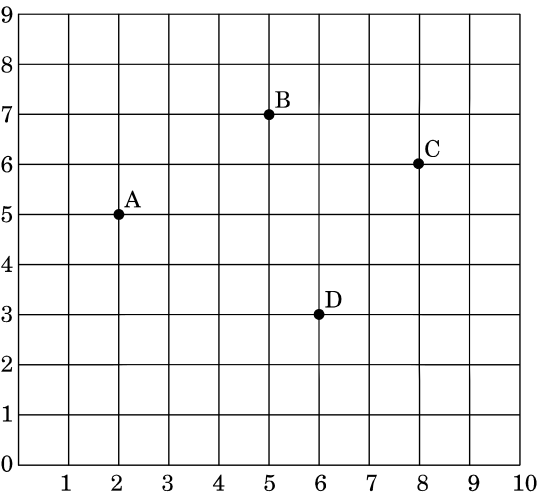
\includegraphics[width=0.45\columnwidth,height=0.45\columnwidth]{figs/fwc3.png}
		     \caption{Based on the above, answer the following question :}
		     \label{fig:my_label}
	     \end{figure}
\begin{enumerate}[label=(\roman*)]
	\item The figure formed by the points $\vec{A}$, $\vec{B}$, $\vec{C}$ and $\vec{D}$ is a
		\begin{enumerate}[label=(\Alph*)]
			\item sqaure
			\item parallelogram
			\item rhombus
			\item quadrilateral
		\end{enumerate}
	\item If the sports teacher is sitting at the origin, then which of the four students is closest to him ?
		\begin{enumerate}[label=(\Alph*)]
			\item $\vec{A}$
			\item $\vec{B}$
			\item $\vec{C}$
			\item $\vec{D}$
		\end{enumerate}
	\item The distance between $\vec{A}$ and $\vec{C}$ is 
		\begin{enumerate}[label=(\Alph*)]
			\item $\sqrt{37}$ units
			\item $\sqrt{35}$ units
			\item $6$ units
			\item $5$ units
		\end{enumerate}
	\item The coordinates of the mid-point of line segment $AC$ are
	\item If a point $\vec{P}$ divides the line segment $AD$ in the ratio $1:2$, then coordinates of $\vec{P}$ are
		\begin{enumerate}[label=(\Alph*)]
			\item $(\frac{8}{3},\frac{8}{3})$
			\item $(\frac{10}{3},\frac{13}{3})$
			\item $(\frac{13}{3},\frac{10}{3})$
			\item $(\frac{16}{3},\frac{11}{3})$
	\end{enumerate}
\end{enumerate}
\item \begin{enumerate}[label=(\alph*)]
		\item Check whether the points $\vec{P}(5, -2)$, $\vec{Q}(6, 4)$ and $\vec{R}(7, -2)$ are the vertices of an isosceles triangle PQR.
		\item Find the ratio in which $\vec{P}(4, 5)$ divides the join of $\vec{A}(2, 3)$ and $\vec{B}(7, 8)$.
\end{enumerate}
\item The coordinate of the three consecutive vertices of a parallelogram ABCD are $\vec{A}(1, 3)$, $\vec{B}(-1, 2)$, and $\vec{C}(2, 5)$. Find the cordinates of the fourth vertex $\vec{D}$.
\item \begin{enumerate}[label=(\alph*)]
		\item If $\vec{P}(2, 2)$, $\vec{Q}(-4, -4)$ and $\vec{R}(5, -8)$ are the vertices of a $\triangle$PQR, then find the length of the median through $\vec{R}$.
		\item Find the ratio in which y-axis divides the line segment joining the points $\vec{A}(5, -6)$ and $\vec{B}(-1, -4)$.Also, find the coordinates of the point of intersection.
\end{enumerate}
\item
	\begin{enumerate}[label=(\alph*)]
		\item Find the ratio in which the line segment joining the points $\vec{A}(1, -5)$ and $\vec{B}(-4, 5)$ is divided by the ax-axis. Also, find coordinates of the point of division.
		\item The points $\vec{A}(0, 3)$, $\vec{B}(-2, a)$ and $\vec{C}(-1, 4)$ are the vertices of a rigth triangle, right-angled at $\vec{A}$. Find the value of a. 
	\end{enumerate}
\end{enumerate}

\subsection{12}

\begin{enumerate}
	\item If $ \vec{a},\vec{b}, \vec{c} $ are position vectors of the points A(2,3,-4), B(3,-4,-5) and C(3,2,-3) respectively, then $ \abs{\vec{a}+\vec{b}+\vec{c}} $ is equal to
		\begin{enumerate}
			\item $\sqrt{113}$
			\item $\sqrt{185}$
			\item $\sqrt{203}$
			\item $\sqrt{209}$
		\end{enumerate}
\item Find the distance of the point (a,b,c) from the x-axis
\item If $ \vec{a}=2\hat{i}-\hat{j}+2\hat{k} $ and $ \vec{b}=5\hat{i}-3\hat{j}-4\hat{k} $, then find the ratio\text{$ \frac{\text{projection of vector  }\vec{a} \text{ on } \vec{b}}{\text{projection of vector } \vec{b} \text{ on vector } \vec{a}} $}
\item Let $\hat{a}$ and $\hat{b}$  be two unit vectors. If the vectors $\vec{c}=\hat{a}+2\hat{b}$ and $\vec{d}=5\hat{a}-4\hat{b}$ are perpendicular to each other, then find the angle between the vectors $\hat{a}$ and $\hat{b}$.
\item Show that $ \abs{\vec{a}} \vec{b}$ + $ \abs{\vec{b}} \vec{a}$ is perpendicular to $\abs{\vec{a} \vec{b}} $- $ \abs{\vec{b}} \vec{a} $, for any two non-zero vectors $\vec{a}$ and $\vec{b}$.
\item Prove that three points A,B and C with position vectors $\vec{a}, \vec{b}$ and $\vec{c}$ respectively are collinear if and only if $( \vec{b} \times \vec{c})+(\vec{c} \times \vec{a})+(\vec{a} \times \vec{b}) = \vec{0}$.
\end{enumerate}
\chapter{Linear Forms}
\section{2023}
\subsection{10}

\begin{enumerate}



  \item \textbf{Assertion (A):} Point $\vec{P}$(0,2) is the point of intersection of $y-axis$ with  the line $3x+2y=4$.\\
    \textbf{Reason (R):} The distance of point $\vec{P}$(0,2) from $x-axis$ is 2 units.


  \item If the pair of equations $3x-y+8=0$ and $6x-ry+16=0$ represent coincident lines, then the value of \text{'$r$'} is:

    \begin{enumerate}
      \item $-\frac{1}{2}$
      \item $\frac{1}{2}$
      \item -2
      \item 2
    \end{enumerate}

  \item The of linear equations $2x=5y+6$ and $15y=6x-18$ represents two lines which are:

      \begin{enumerate}
        \item intersecting
        \item parallel
        \item coincident
        \item either intersecting or parallel
      \end{enumerate}

    \item Find the equations of the diagonals of the parallelogram $\vec{PQRS}$ whose vertices are $\vec{P}$(4,2,-6), $\vec{Q}$(5,-3,1), $\vec{R}$(12,4,5) and $\vec{S}$(11,9,-2). Use these equations to find the point of intersection of diagonals.

  \item A line $l$ passes through point (-1,3,-2) and is perpendicular to both the lines $\frac {x}{1}=\frac{y}{2}=\frac{z}{3}$ and $\frac {x+2}{-3}=\frac{y-1}{2}=\frac{z+1}{5}$. Find the ctor equation of the line $l$. Hence, obtain its distance from origin.

\end{enumerate}

\subsection{12}                                                                                                  
\documentclass[12pt,A4 paper]{article}
\usepackage{mathtools}
\usepackage{graphicx}
\usepackage{gensymb}
\begin{document}
\title{\textbf{LINEAR}}
\date{}
\maketitle
\begin{enumerate}
    \item Equation of line passing through origin and making $30\degree,60\degree$ and $90\degree$ with $x,y,z$ axes respectively is
    \begin{enumerate}
        \item $\frac{2x}{\sqrt3}=\frac{y}{2}=\frac{z}{0}$
        \item $\frac{2x}{\sqrt3}=\frac{2y}{1}=\frac{z}{0}$
        \item $2x=\frac{2y}{\sqrt3}=\frac{z}{1}$
        \item $\frac{2x}{\sqrt3}=\frac{2y}{1}=\frac{z}{1}$
    \end{enumerate}
    \item If the equation of a line is $x=ay+b,z=cy+d$,then find the direction ratios of the line and a point on the line.
    \item
    \begin{enumerate}
        \item Find the equations of the diagonals of the parallelogram $PQRS$ whose vertices are$P(4,2,-6),Q(5,-3,1),R(12,4,5),S(11,9,-2)$.Use these equations to find the point of intersection of diagonals.  
        \item A line $l$ passes through point$(-1,3,-2)$ and is perpendicular to both the lines $\frac{x}{1}=\frac{y}{2}=\frac{z}{3}$ and $\frac{x+2}{-3}=\frac{y-1}{2}=\frac{z+1}{5}$.Find the vector equation of the line $l$.Hence,obtain its distance from origin.
    \end{enumerate}
   
   
   
\end{enumerate}
\end{document}


\section{2022}
\begin{enumerate}[label=\thesection.\arabic*.,ref=\thesection.\theenumi]
\numberwithin{equation}{enumi}
\numberwithin{figure}{enumi}
\numberwithin{table}{enumi}

\item Solve the equations $x+2y=6$ and $2x-5y=12$ graphically.	

	\item Solve the following equations for $x$ and $y$ using cross-multiplication method:
		\begin{align}
			(ax-by)+(a+4b)=0\\(bx+ay)+(b-4a)=0
		\end{align}

	\item Find the co-ordinates of the point where the line $\dfrac{x-3}{-1}=\dfrac{y+4}{1}=\dfrac{z+5}{6}$ crosses the plane passing through the points $\left(\dfrac{7}{2},0,0\right),(0,7,0),(0,0,7)$.

	\item Electrical transmission wires which are laid down in winters are stretched tightly to accommodate expansion in summers.
		\begin{figure}[H]
			\centering
			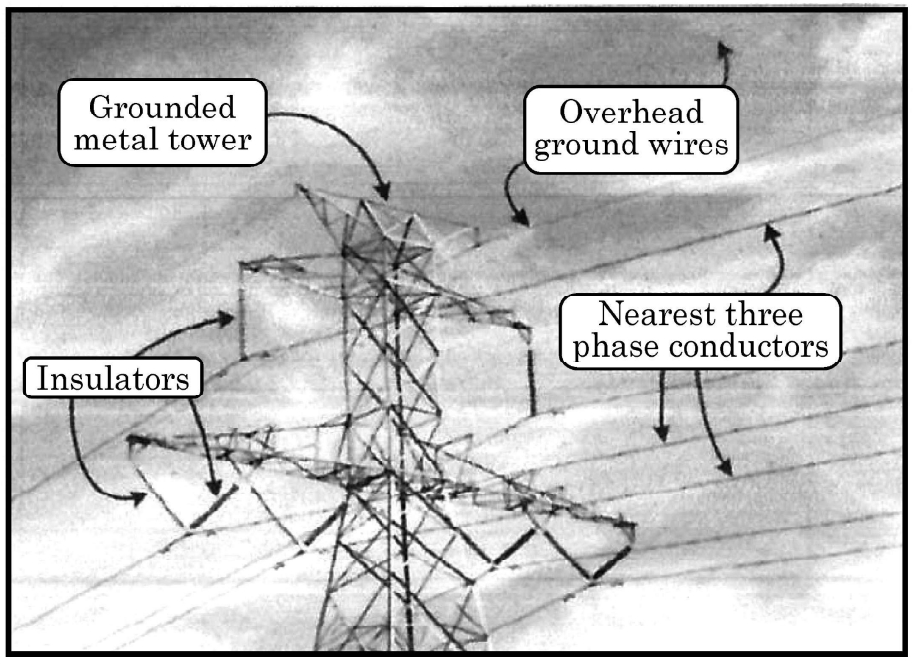
\includegraphics[width=\columnwidth]{figs/txn}
			\caption{Electrical transmission wires connected to a transmission tower.}
			\label{fig:txn1}
		\end{figure}
		Two such wires in the figure \ref{fig:txn1} lie along the following lines:
		\begin{align}
			l_1 &: \dfrac{x+1}{3}=\dfrac{y-3}{-2}=\dfrac{z+2}{-1}\\
			l_2 &: \dfrac{x}{-1}=\dfrac{y-7}{3}=\dfrac{z+7}{-2}
		\end{align}
		Based on the given information, answer the following questions:
		\begin{enumerate}
			\item	Are the $l_1$ and $l_2$ coplanar? Justify your answer.
			\item    Find the point of intersection of lines $l_1$ and $l_2$.
		\end{enumerate}

	\item Write the cartesian equation of the line PQ passing through points P$(2,2,1)$ and Q$(5,1,-2)$. Hence, find the y-coordinate of the point on the line PQ whose z-coordinate is -2.

	\item Find the distance between the lines $x=\dfrac{y-1}{2}=\dfrac{z-2}{3}$ and $x+1=\dfrac{y+2}{2}=\dfrac{z-1}{3}$.
	
	\item Find the shortest distance between the following lines:
		\begin{align}
			\vec{r}&=3\hat{i}+5\hat{j}+7\hat{k}+\lambda(\hat{i}-2\hat{j}+\hat{k})\\\vec{r}&=(-\hat{i}-\hat{j}-\hat{k})+\mu(7\hat{i}-6\hat{j}+\hat{k})
		\end{align}

	\item Two motorcycles A and B are running at a speed more than the allowed speed on the road (as shown in figure \ref{fig:bike1}) represented by the following lines 
		\begin{align}
			\vec{r}&=\lambda(\hat{i}+2\hat{j}-\hat{k})\\\vec{r}&=(3\hat{i}+3\hat{j})+\mu(2\hat{i}+\hat{j}+\hat{k})
		\end{align}
		\begin{figure}[H]
			\centering
			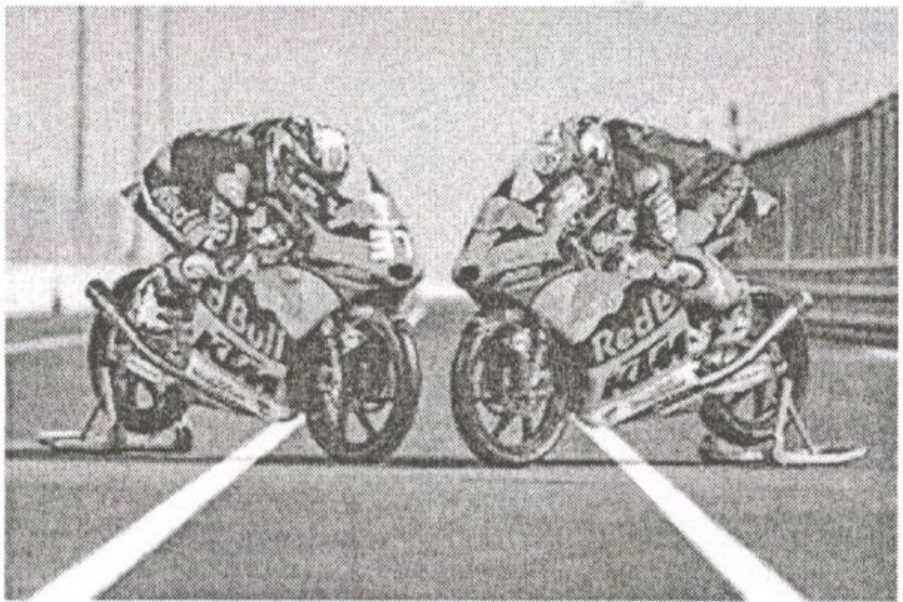
\includegraphics[width=\columnwidth]{figs/bike}
			\caption{Two motorcycles moving along the road in a straight line.}
			\label{fig:bike1}
		\end{figure}
		Based on the following information, answer the following questions:
		\begin{enumerate}
			\item Find the shortest distance between the given lines.
			\item Find a point at which the motorcycles may collide.
		\end{enumerate}
	
	\item Find the shortest distance between the following lines
		\begin{align}
			\vec{r}&=(\lambda+1)\hat{i}+(\lambda+4)\hat{j}-(\lambda-3)\hat{k}\\\vec{r}&=(3-\mu)\hat{i}+(2\mu+2)\hat{j}+(\mu+6)\hat{k}
		\end{align}
	
	\item Find the shortest distance between the following lines and hence write whether the lines are intersecting or not.
		\begin{align}
			\dfrac{x-1}{2}=\dfrac{y+1}{3}=z, \dfrac{x+1}{5}=\dfrac{y-2}{1}, z=2
		\end{align}

		\item Find the equation of the plane passing through the points $(2,1,0),(3,-2,-2)$ and $(1,1,7)$. Also, obtain its distance from the origin.

	\item The foot of a perpendicular drawn from the point $(-2,-1,-3)$ on a plane is $(1,-3,3)$. Find the equation of the plane.

	\item Find the cartesian and the vector equation of a plane which passes through the point $(3,2,0)$ and contains the line $\dfrac{x-3}{1}=\dfrac{y-6}{5}=\dfrac{z-4}{4}$.

	\item The distance between the planes $4x-4y+2z+5=0$ and $2x-2y+z+6=0$ is

		\begin{enumerate}

			\item $\dfrac{1}{6}$
			\item $\dfrac{7}{6}$
			\item $\dfrac{11}{6}$
			\item $\dfrac{16}{6}$
		\end{enumerate}

	\item Find the equation of the plane through the line of intersection of the planes
		\begin{align}
			\vec{r}\cdot(\hat{i}+3\hat{j})+6&=0\\\vec{r}\cdot(3\hat{i}-\hat{j}-4\hat{k})&=0
		\end{align}which is at a  unit distance from the origin.

		\item If the distance of the point $(1,1,1)$ from the plane $x-y+z+\lambda=0$ is $\dfrac{5}{\sqrt{3}}$, find the value(s) of $\lambda$.

	\item Find the distance of the point $(2,3,4)$ measured along the line $\dfrac{x-4}{3}=\dfrac{y+5}{6}=\dfrac{z+1}{2}$ from the plane $3x+2y+2z+5=0$.

	\item Find the distance of the point $P(4,3,2)$ from the plane determined by the points $A(-1,6,-5),B(-5,-2,3)$ and $C(2,4,-5)$.

	\item The distance of the line
		\begin{align}
		\vec{r}=(\hat{i}-\hat{j})+\lambda(\hat{i}+5\hat{j}+\hat{k})\end{align}
		from the plane
		\begin{align}
		\vec{r}\cdot(\hat{i}-\hat{j}+4\hat{k})=5\end{align}
		is
		\begin{enumerate}
			\item $\sqrt{2}$
			\item $\dfrac{1}{\sqrt{2}}$
			\item $\dfrac{1}{3\sqrt{2}}$
			\item $\dfrac{-2}{3\sqrt{2}}$
		\end{enumerate}

	\item Find a unit vector perpendicular to each of the vectors $(\vec{a}+\vec{b})$ and $(\vec{a}-\vec{b})$ where 
	\begin{align}
		\vec{a}&=\hat{i}+\hat{j}+\hat{k}\\\vec{b}&=\hat{i}+2\hat{j}+3\hat{k}
	\end{align}

	\item Find the distance of the point $(1,-2,9)$ from the point of intersection of the line
		\begin{align}
			\vec{r}=4\hat{i}+2\hat{j}+7\hat{k}+\lambda(3\hat{i}+4\hat{j}+2\hat{k})
		\end{align}and the plane
		\begin{align}
			\vec{r}\cdot(\hat{i}-\hat{j}+\hat{k})=10.
		\end{align}

	\item Find the area bounded by the curves $y=\abs{x-1}$ and $y=1$, using integration.

	\item Find the coordinates of the point where the line through $(4,-3,-4)$ and $(3,-2,2)$ crosses the plane $2x+y+z=6$.

	\item Fit a straight line trend by the method of least squares and find the trend value for the year 2008 using the data from Table \ref{tab:LC}:
		\begin{table}[H]
			\caption{Table showing yearly trend of production of goods in lakh tonnes \label{tab:LC}}
			%%%%%%%%%%%%%%%%%%%%%%%%%%%%%%%%%%%%%%%%%%%%%%%%%%%%%%%%%%%%%%%%%%%%%%
%%                                                                  %%
%%  This is the header of a LaTeX2e file exported from Gnumeric.    %%
%%                                                                  %%
%%  This file can be compiled as it stands or included in another   %%
%%  LaTeX document. The table is based on the longtable package so  %%
%%  the longtable options (headers, footers...) can be set in the   %%
%%  preamble section below (see PRAMBLE).                           %%
%%                                                                  %%
%%  To include the file in another, the following two lines must be %%
%%  in the including file:                                          %%
%%        \def\inputGnumericTable{}                                 %%
%%  at the beginning of the file and:                               %%
%%        \input{name-of-this-file.tex}                             %%
%%  where the table is to be placed. Note also that the including   %%
%%  file must use the following packages for the table to be        %%
%%  rendered correctly:                                             %%
%%    \usepackage[latin1]{inputenc}                                 %%
%%    \usepackage{color}                                            %%
%%    \usepackage{array}                                            %%
%%    \usepackage{longtable}                                        %%
%%    \usepackage{calc}                                             %%
%%    \usepackage{multirow}                                         %%
%%    \usepackage{hhline}                                           %%
%%    \usepackage{ifthen}                                           %%
%%  optionally (for landscape tables embedded in another document): %%
%%    \usepackage{lscape}                                           %%
%%                                                                  %%
%%%%%%%%%%%%%%%%%%%%%%%%%%%%%%%%%%%%%%%%%%%%%%%%%%%%%%%%%%%%%%%%%%%%%%



%%  This section checks if we are begin input into another file or  %%
%%  the file will be compiled alone. First use a macro taken from   %%
%%  the TeXbook ex 7.7 (suggestion of Han-Wen Nienhuys).            %%
\def\ifundefined#1{\expandafter\ifx\csname#1\endcsname\relax}


%%  Check for the \def token for inputed files. If it is not        %%
%%  defined, the file will be processed as a standalone and the     %%
%%  preamble will be used.                                          %%
\ifundefined{inputGnumericTable}

%%  We must be able to close or not the document at the end.        %%
 \def\gnumericTableEnd{\end{document}}


%%%%%%%%%%%%%%%%%%%%%%%%%%%%%%%%%%%%%%%%%%%%%%%%%%%%%%%%%%%%%%%%%%%%%%
%%                                                                  %%
%%  This is the PREAMBLE. Change these values to get the right      %%
%%  paper size and other niceties.                                  %%
%%                                                                  %%
%%%%%%%%%%%%%%%%%%%%%%%%%%%%%%%%%%%%%%%%%%%%%%%%%%%%%%%%%%%%%%%%%%%%%%

 \documentclass[12pt%
     %,landscape%
                    ]{report}
       \usepackage[latin1]{inputenc}
       \usepackage{fullpage}
       \usepackage{color}
       \usepackage{array}
       \usepackage{longtable}
       \usepackage{calc}
       \usepackage{multirow}
       \usepackage{hhline}
       \usepackage{ifthen}

 \begin{document}


%%  End of the preamble for the standalone. The next section is for %%
%%  documents which are included into other LaTeX2e files.          %%
\else

%%  We are not a stand alone document. For a regular table, we will %%
%%  have no preamble and only define the closing to mean nothing.   %%
    \def\gnumericTableEnd{}

%%  If we want landscape mode in an embedded document, comment out  %%
%%  the line above and uncomment the two below. The table will      %%
%%  begin on a new page and run in landscape mode.                  %%
%       \def\gnumericTableEnd{\end{landscape}}
%       \begin{landscape}


%%  End of theelse clause for this file being \input.              %%
\fi

%%%%%%%%%%%%%%%%%%%%%%%%%%%%%%%%%%%%%%%%%%%%%%%%%%%%%%%%%%%%%%%%%%%%%%
%%                                                                  %%
%%  The rest is the gnumeric table, except for the closing          %%
%%  statement. Changes below will alter the table's appearance.     %%
%%                                                                  %%
%%%%%%%%%%%%%%%%%%%%%%%%%%%%%%%%%%%%%%%%%%%%%%%%%%%%%%%%%%%%%%%%%%%%%%

\providecommand{\gnumericmathit}[1]{#1} 
%%  Uncomment the next line if you would like your numbers to be in %%
%%  italics if they are italizised in the gnumeric table.           %%
%\renewcommand{\gnumericmathit}[1]{\mathit{#1}}
\providecommand{\gnumericPB}[1]%
{\let\gnumericTemp=\\#1\let\\=\gnumericTemp\hspace{0pt}}
 \ifundefined{gnumericTableWidthDefined}
        \newlength{\gnumericTableWidth}
        \newlength{\gnumericTableWidthComplete}
        \newlength{\gnumericMultiRowLength}
        \global\def\gnumericTableWidthDefined{}
 \fi
%% The following setting protects this code from babel shorthands.  %%
 \ifthenelse{\isundefined{\languageshorthands}}{}{\languageshorthands{english}}
%%  The default table format retains the relative column widths of  %%
%%  gnumeric. They can easily be changed to c, r or l. In that case %%
%%  you may want to comment out the next line and uncomment the one %%
%%  thereafter                                                      %%
\providecommand\gnumbox{\makebox[0pt]}
%%\providecommand\gnumbox[1][]{\makebox}

%% to adjust positions in multirow situations                       %%
\setlength{\bigstrutjot}{\jot}
\setlength{\extrarowheight}{\doublerulesep}

%%  The \setlongtables command keeps column widths the same across  %%
%%  pages. Simply comment out next line for varying column widths.  %%
\setlongtables

\setlength\gnumericTableWidth{%
 53pt+%
 53pt+%
 106pt+%
0pt}
\def\gumericNumCols{3}
\setlength\gnumericTableWidthComplete{\gnumericTableWidth+%
         \tabcolsep*\gumericNumCols*2+\arrayrulewidth*\gumericNumCols}
\ifthenelse{\lengthtest{\gnumericTableWidthComplete > \linewidth}}%
         {\def\gnumericScale{\ratio{\linewidth-%
                        \tabcolsep*\gumericNumCols*2-%
                        \arrayrulewidth*\gumericNumCols}%
{\gnumericTableWidth}}}%
{\def\gnumericScale{1}}

%%%%%%%%%%%%%%%%%%%%%%%%%%%%%%%%%%%%%%%%%%%%%%%%%%%%%%%%%%%%%%%%%%%%%%
%%                                                                  %%
%% The following are the widths of the various columns. We are      %%
%% defining them here because then they are easier to change.       %%
%% Depending on the cell formats we may use them more than once.    %%
%%                                                                  %%
%%%%%%%%%%%%%%%%%%%%%%%%%%%%%%%%%%%%%%%%%%%%%%%%%%%%%%%%%%%%%%%%%%%%%%

\ifthenelse{\isundefined{\gnumericColA}}{\newlength{\gnumericColA}}{}\settowidth{\gnumericColA}{\begin{tabular}{@{}p{53pt*\gnumericScale}@{}}x\end{tabular}}
\ifthenelse{\isundefined{\gnumericColB}}{\newlength{\gnumericColB}}{}\settowidth{\gnumericColB}{\begin{tabular}{@{}p{150pt*\gnumericScale}@{}}x\end{tabular}}
\ifthenelse{\isundefined{\gnumericColC}}{\newlength{\gnumericColC}}{}\settowidth{\gnumericColC}{\begin{tabular}{@{}p{106pt*\gnumericScale}@{}}x\end{tabular}}

\begin{longtable}[c]{%
 b{\gnumericColA}%
 b{\gnumericColB}%
 b{\gnumericColC}%
 }

%%%%%%%%%%%%%%%%%%%%%%%%%%%%%%%%%%%%%%%%%%%%%%%%%%%%%%%%%%%%%%%%%%%%%%
%%  The longtable options. (Caption, headers... see Goosens, p.124) %%
% \caption{The Table Caption.}             \\ %
% \hline % Across the top of the table.
%%  The rest of these options are table rows which are placed on    %%
%%  the first, last or every page. Use \multicolumn if you want.    %%

%%  Header for the first page.                                      %%
% \multicolumn{3}{c}{The First Header} \\ \hline 
% \multicolumn{1}{c}{colTag} %Column 1
% &\multicolumn{1}{c}{colTag} %Column 2
% &\multicolumn{1}{c}{colTag} \\ \hline %Last column
% \endfirsthead

%%  The running header deinition.

%%
% \hline
% \multicolumn{3}{l}{\ldots\small\slshape continued} \\ \hline
% \multicolumn{1}{c}{colTag} %Column 1
% &\multicolumn{1}{c}{colTag} %Column 2
% &\multicolumn{1}{c}{colTag} \\ \hline %Last column
% \endhead

%%  The running footer definition.                                  %%
% \hline
% \multicolumn{3}{r}{\small\slshape continued\ldots} \\
% \endfoot

%%  The ending footer definition.                                   %%
% \multicolumn{3}{c}{That's all folks} \\ \hline 
% \endlastfoot
%%%%%%%%%%%%%%%%%%%%%%%%%%%%%%%%%%%%%%%%%%%%%%%%%%%%%%%%%%%%%%%%%%%%%%

\hhline{|-|-|-}
  \multicolumn{1}{|p{\gnumericColA}|}%
 {\gnumericPB{\raggedright}\gnumbox[l]{Year}}
 &\multicolumn{1}{p{\gnumericColB}|}%
	{\gnumericPB{\raggedright}\gnumbox[l]{Production (in lakh tonnes)}}
 %&\multicolumn{1}{p{\gnumericColC}|}%
 %{\gnumericPB{\raggedright}\gnumbox[l]{Description}}
\\
\hhline{|---|}
  \multicolumn{1}{|p{\gnumericColA}|}%
 {\gnumericPB{\raggedright}\gnumbox[l]{2001}}
 &\multicolumn{1}{p{\gnumericColB}|}%
 {\gnumericPB{\raggedright}\gnumbox[l]{30}}
 %&\multicolumn{1}{p{\gnumericColC}|}%
 %{\gnumericPB{\raggedright}\gnumbox[l]{Vertex A}}
\\
\hhline{|---|}
  \multicolumn{1}{|p{\gnumericColA}|}%
 {\gnumericPB{\raggedright}\gnumbox[l]{2002}}
 &\multicolumn{1}{p{\gnumericColB}|}%
 {\gnumericPB{\raggedright}\gnumbox[l]{35}}
 %&\multicolumn{1}{p{\gnumericColC}|}%
 %{\gnumericPB{\raggedright}\gnumbox[l]{Vertex B}}
\\
\hhline{|---|}
  \multicolumn{1}{|p{\gnumericColA}|}%
 {\gnumericPB{\raggedright}\gnumbox[l]{2003}}
 &\multicolumn{1}{p{\gnumericColB}|}%
 {\gnumericPB{\raggedright}\gnumbox[l]{36}}
 %&\multicolumn{1}{p{\gnumericColC}|}%
 %{\gnumericPB{\raggedright}\gnumbox[l]{Vertex C}}
\\
\hhline{|---|}
  \multicolumn{1}{|p{\gnumericColA}|}%
 {\gnumericPB{\raggedright}\gnumbox[l]{2004}}
 &\multicolumn{1}{p{\gnumericColB}|}%
 {\gnumericPB{\raggedright}\gnumbox[l]{32}}
 %&\multicolumn{1}{p{\gnumericColC}|}%
 %{\gnumericPB{\raggedright}\gnumbox[l]{Midpoint of AC}}
\\
\hhline{|---|}
  \multicolumn{1}{|p{\gnumericColA}|}%
 {\gnumericPB{\raggedright}\gnumbox[l]{2005}}
 &\multicolumn{1}{p{\gnumericColB}|}%
 {\gnumericPB{\raggedright}\gnumbox[l]{37}}
 %&\multicolumn{1}{p{\gnumericColC}|}%
 %{\gnumericPB{\raggedright}\gnumbox[l]{Midpoint of BC}}
\\
\hhline{|---|}
  \multicolumn{1}{|p{\gnumericColA}|}%
 {\gnumericPB{\raggedright}\gnumbox[l]{2006}}
 &\multicolumn{1}{p{\gnumericColB}|}%
 {\gnumericPB{\raggedright}\gnumbox[l]{40}}
 %&\multicolumn{1}{p{\gnumericColC}|}%
 %{\gnumericPB{\raggedright}\gnumbox[l]{Midpoint of AB}}
\\
\hhline{|-|-|-|}
\end{longtable}

\ifthenelse{\isundefined{\languageshorthands}}{}{\languageshorthands{\languagename}}
\gnumericTableEnd

		\end{table}
\end{enumerate}

\section{2021}
\subsection{10}
%\documentclass{article}
%\let\vec\mathbf
%\usepackage{graphicx}
%\usepackage{amsmath}
%\usepackage{gensymb}
%\usepackage{float}
%\graphicspath{{./documents/}{./figs}}
%\begin{document}
\begin{enumerate}[label=\thesection.\arabic*.,ref=\thesection.\theenumi]
\numberwithin{equation}{enumi}
\numberwithin{figure}{enumi}
\numberwithin{table}{enumi}
	\item If the graph of a pair of lines $ x - 2y + 3 = 0 $ and $ 2x - 4y = 5 $ be drawn, that what type of lines are drawn ? 
\end{enumerate}
%\end{document}

\subsection{12}
\begin{enumerate}
    \item If the two lines
    \begin{align}
          L_1 : x=5,\frac{y}{3-\alpha}=\frac{z}{-2}\\
         L_1 : x=2,\frac{y}{-1}=\frac{z}{z-\alpha} 
       \end{align}
  are perpendicular,then the value of $\alpha$ 
        \begin{enumerate}
        \item $\frac{2}{3}$
        \item $3$
        \item $4$
        \item $\frac{7}{3}$
    \end{enumerate}

    \item Find the shortest distance between the following lines and hence write
whether the lines are intersecting or not.
\begin{align}
    \frac{x-1}{2} &= \frac{y+1}{3} = z \\
    \frac{x+1}{5} &=\frac{y-2}{1},z=2
\end{align}

\item  Find the equation of the plane through the line of intersection of the planes 
\begin{align}
     \vec{r} .\brak{i+3j} + 6 &= 0 \\  \vec{r} .\brak{3i - j - 4k} &= 0
\end{align}
which is at a unit distance from the origin.
    \item If segment of the line intercepted between the co-ordinate-axes is bisected
at the point $M\brak{2, 3}$, then the equation of this line is
 \begin{align}
       2x + 3y &= 13\\
       x + y &= 5 \\
       2x + y &= 7\\
       3x + 2y &= 12
\end{align}
\item The equation of a line through $(2,-4)$ and parallel to x-axis is $\underline{\hspace{2cm}}$.
\item Find the equation of the median through vertex $A$ of the triangle $ABC$, having vertices $A\brak{2,5}$, $B\brak{-4,9}$ and $C\brak{-2, -1}$.
\item Solve the system of linear equations, using matrix method : 
\begin{align}
  7x + 2y &= 11\\
 4x - y &= 2
\end{align}
\end{enumerate}

\chapter{Circles}
\section{2023}
\subsection{10}
%\documentclass{article}
%\usepackage{gensymb}
%\let\vec\mathbf
%\usepackage{float}
%\usepackage{graphicx}
%\newcommand\figref{Fig.~\ref}
%\graphicspath{{./Documents}}
%\begin{document}
\begin{enumerate}
	\item In the given figure \figref{fig:circle1}, $ PQ $ is tangent to the circle centred at $ \vec{O} $. If $ \angle{AOB} = 95{\degree} $, then measure of $ \angle{ABQ} $ will be
	\begin{figure}[H]
		\centering
		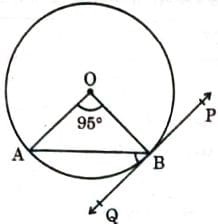
\includegraphics[width=\columnwidth]{figs/fig1.jpg}
		\caption{}
		\label{fig:circle1}
	\end{figure}
		\begin{enumerate}
			\item $ 47.5{\degree} $
			\item $ 42.5{\degree} $
			\item $ 85{\degree} $
			\item $ 95{\degree} $
		\end{enumerate}
	\item
		\begin{enumerate}
			\item In the given figure \figref{fig:circle2}, two tangents $ TP $ and $ TQ $ are drawn to be a circle with centre $ \vec{O} $ from an external point $ \vec{T} $. Prove that $ \angle{PTQ} = 2\angle{OPQ} $.
		\begin{figure}[H]
			\centering
			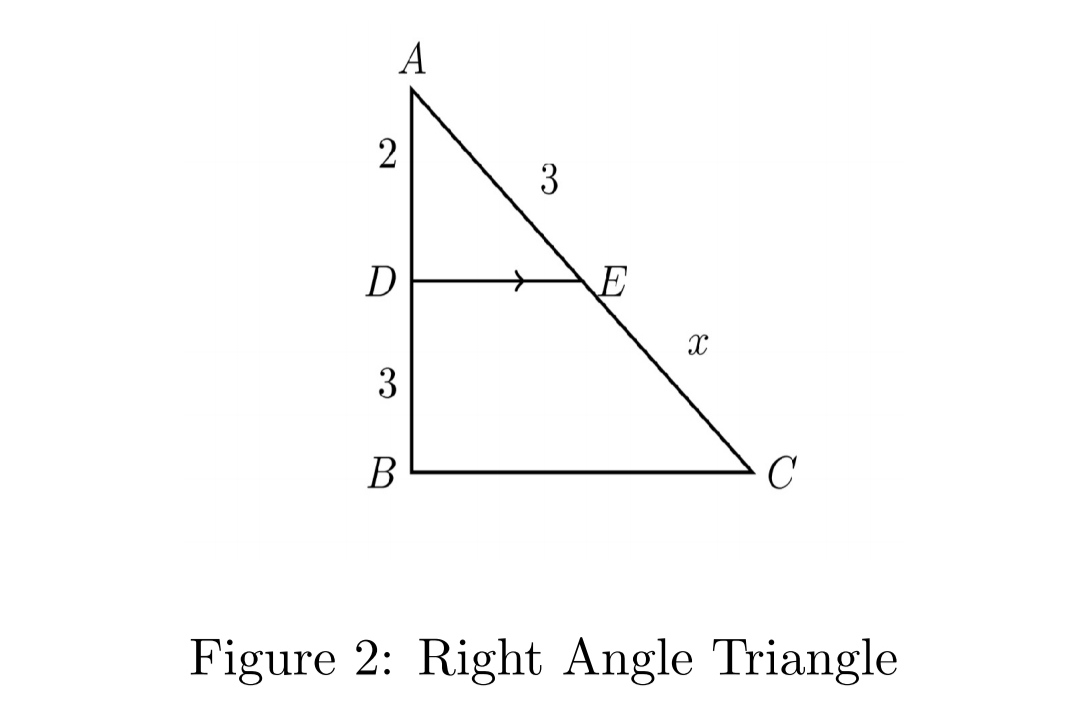
\includegraphics[width=\columnwidth]{figs/fig2.jpg}
			\caption{}
			\label{fig:circle2}
		\end{figure}
	\item In the given figure \figref{fig:circle3}, a circle is inscribed in a quadrilateral $ ABCD $ in which $ \angle{B} = 90{\degree} $. If $ AD = 17 cm, AB = 20 cm $ and $ DS = 3cm $, then find the radius of the circle.
		\begin{figure}[H]
			\centering 
			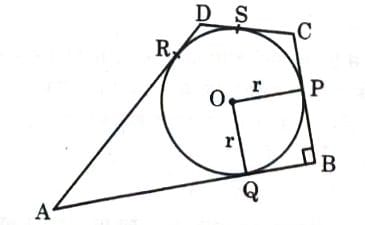
\includegraphics[width=\columnwidth]{figs/fig3.jpg}
			\caption{}
			\label{fig:circle3}
		\end{figure}
		\end{enumerate}
	\item The discus throw is an event in which an athlete attempts to throw a discus. The athlete spins anti-clockwise around one and a half times through a cicrle as shown in \figref{fig:tangentline} below, then releases the throw. When released, the discus travels along tangent to the circular spin orbit.
		\begin{figure}[H]
			\centering
			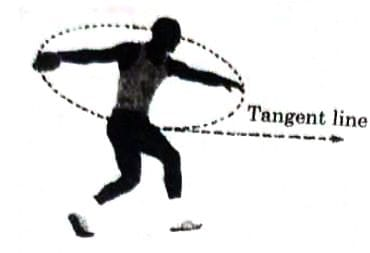
\includegraphics[width=\columnwidth]{figs/fig4.jpg}
			\caption{}
			\label{fig:tangentline}
		\end{figure}
		In the given figure \figref{fig:circle5}, $ AB $ is one such tangent to a circle of radius 75 cm. Point $ \vec{O} $ is centre of the circle and $ \angle{ABO} = 30{\degree} . PQ $ is parallel to $ OA $.
		\begin{figure}[H]
			\centering
			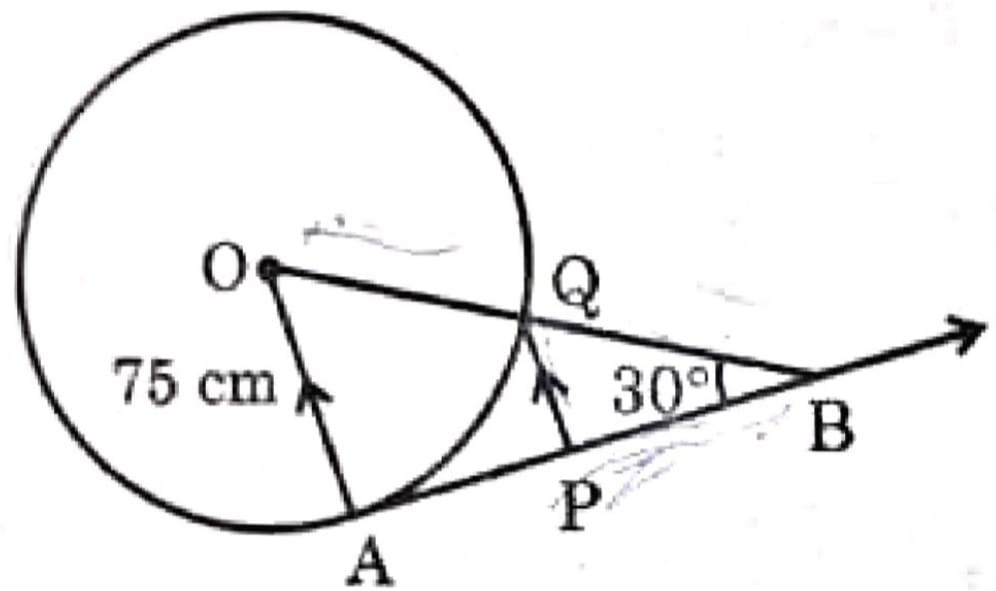
\includegraphics[width=\columnwidth]{figs/fig5.jpg}
			\caption{}
			\label{fig:circle5}
		\end{figure}
		Based on above information :
		\begin{enumerate}
			\item find the length of $ AB $.
			\item find the length of $ OB $.
			\item find the length of $ AP $.
			\item find the length of $ PQ $.
		\end{enumerate}
	\item In the given figure \figref{fig:circle6}, the quadrilateral $ PQRS $ circumscribes a circle. Here $ PA + CS $ is equal to :
		\begin{figure}[H]
			\centering
			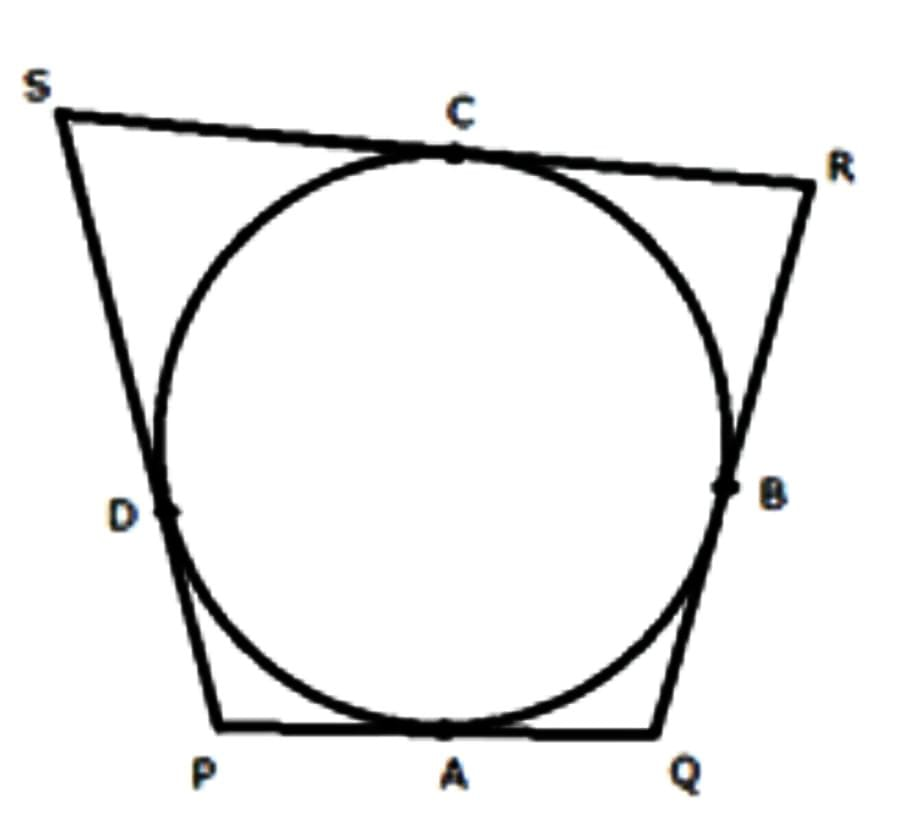
\includegraphics[width=\columnwidth]{figs/fig6.jpg}
			\caption{}
			\label{fig:circle6}
		\end{figure}
		\begin{enumerate}
			\item $ QR $
			\item $ PR $
			\item $ PS $
			\item $ PQ $
		\end{enumerate}
	\item In the given figure \figref{fig:circle7}, $ \vec{O} $ is the centre of the circle. $ AB $ and $ AC $ are tangents drawn to the circle from point $ \vec{A} $. If $ \angle{BAC} = 65{\degree} $, then find the measure of $ \angle{BOC} $.
		\begin{figure}[H]
			\centering
			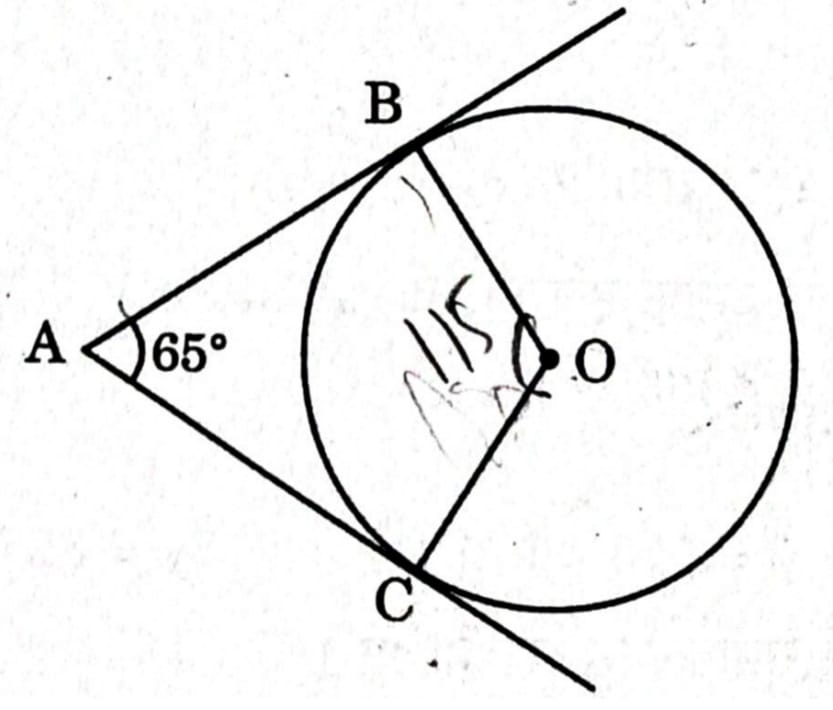
\includegraphics[width=\columnwidth]{figs/fig7.jpg}
			\caption{}
			\label{fig:circle7}
		\end{figure}
	\item In the given figure \figref{fig:circle8}, $ \vec{O} $ is the centre of the circle and $ QPR $ is the tangent to it at $ \vec{P} $. Prove that $ \angle{QAP} + \angle{APR} = 90{\degree} $.			
		\begin{figure}[H]
			\centering
			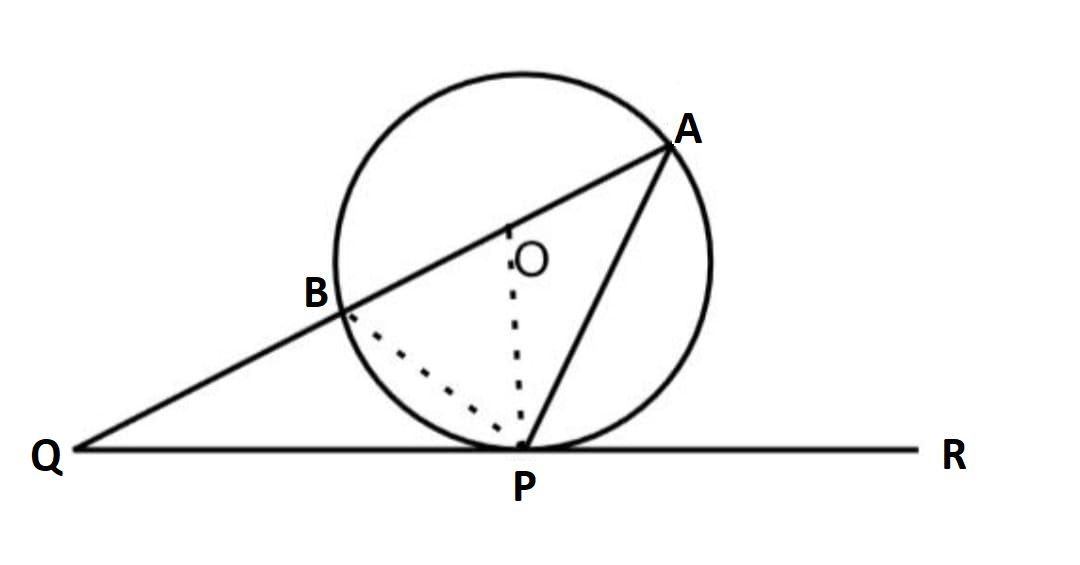
\includegraphics[width=\columnwidth]{figs/fig8.jpg}
			\caption{}
			\label{fig:circle8}
		\end{figure}
	\item In the given figure \figref{fig:circle9}, $ TA $ is a tangent to the circle with centre $ \vec{O} $ such that $ OT = 4 cm , \angle{OTA} = 30{\degree} $, then length of $ TA $ is :
		\begin{figure}[H]
			\centering
			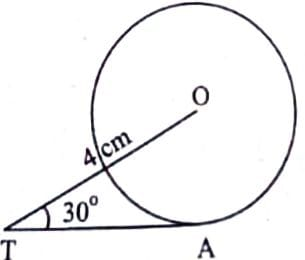
\includegraphics[width=\columnwidth]{figs/fig9.jpg}
			\caption{}
			\label{fig:circle9}
		\end{figure}
		\begin{enumerate}
			\item $ 2\sqrt{3} cm $
			\item $ 2 cm $
			\item $ 2\sqrt{2} cm $
			\item $ \sqrt{3} cm $
		\end{enumerate}
	\item In the given figure \figref{fig:circle10}, $ PT $ is a tangent at $ \vec{T} $ to the circle with centre $ \vec{O} $. If $ \angle{TPO} = 25{\degree} $, then $ x $ is equal to : 	
		\begin{figure}[H]
			\centering
			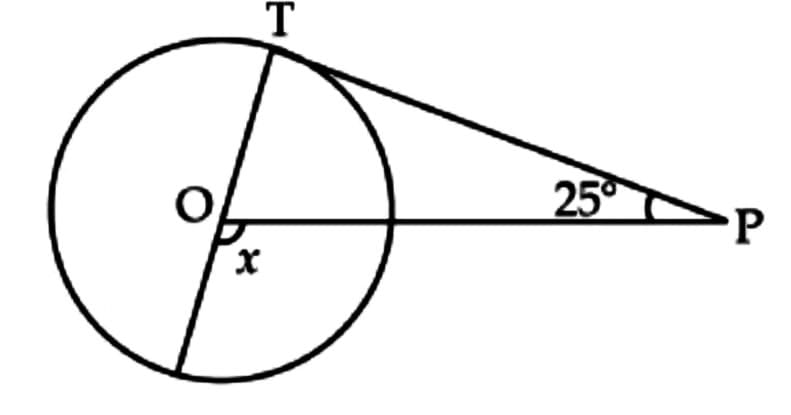
\includegraphics[width=\columnwidth]{figs/fig10.jpg}
			\caption{}
			\label{fig:circle10}
		\end{figure}
		\begin{enumerate}
			\item $ 25{\degree} $
			\item $ 65{\degree} $
			\item $ 90{\degree} $
			\item $ 115{\degree} $
		\end{enumerate}
	\item Two concentric circles are of radii 5 cm and 3 cm. Find the length of the chord of the larger circle which touches the smaller circle.
\end{enumerate}
%\end{document}

\section{2022}
\begin{enumerate}[label=\thesection.\arabic*.,ref=\thesection.\theenumi]
\numberwithin{equation}{enumi}
\numberwithin{figure}{enumi}
\numberwithin{table}{enumi}

	\item Draw a circle of radius 2.5 cm. Take a point $\vec{P}$ outside the circle at a distance of 7 cm from the center. Then construct a pair of tangents to the circle from point $\vec{P}$.

	\item Write the steps of construction for constructing a pair of tangents to a circle of radius 4 cm from a point $\vec{P}$, at a distance of 7 cm from its center $\vec{O}$.

	\item In Figure \ref{fig:tan1}, there are two concentric circles with centre $\vec{O}$. If $ARC$ and $AQB$ are tangents to the smaller circle  from the point $\vec{A}$ lying on the larger circle, find the length of $AC$, if $AQ$ = 5 cm.
		\begin{figure}[H]
			\centering
			
\includegraphics[width=\columnwidth]{figs/tan}
			\caption{Two concentric circles with $\vec{O}$ as centre}
			\label{fig:tan1}
		\end{figure}
	
	\item In Figure \ref{fig:cir1}, if a circle touches the side $QR$ of $\Delta PQR$ at $\vec{S}$ and extended sides $PQ$ and $PR$ at $\vec{M}$ and $\vec{N}$, respectively,
		\begin{figure}[H]
			\centering
			
\includegraphics[width=\columnwidth]{figs/cir}
				\caption{Two tangents are drawn from point $\vec{P}$ to the circle}
				\label{fig:cir1}
		\end{figure}
		prove that $PM=\dfrac{1}{2}(PQ+QR+PR)$

	\item In Figure \ref{fig:tri1}, a triangle $ABC$ is drawn to circumscribe a circle of radius 4 cm such that the segments $BD$ and $DC$ into which $BC$ is divided by the point of contact $\vec{D}$ are of lengths 6 cm and 8 cm respectively. If the area of $\Delta ABC$ is 84 $cm^2$, find the lengths of sides $AB$ and $AC$.
		\begin{figure}[H]
			\centering
			
\includegraphics[width=\columnwidth]{figs/tri}
				\caption{Circle with $\vec{O}$ as center circumscribed in triangle $ABC$}
				\label{fig:tri1}
		\end{figure}

	\item In Figure \ref{fig:sq1}, $PQ$ and $PR$ are tangents to the circle centered at $\vec{O}$. If $\angle OPR=45\degree$, then prove that $ORPQ$ is a square.
		\begin{figure}[H]
			\centering
			
\includegraphics[width=\columnwidth]{figs/sq}
			\caption{Two tangents drawn from point $\vec{P}$ to a circle whose centre is $\vec{O}$}
			\label{fig:sq1}
		\end{figure}

	\item In Figure \ref{fig:sct1}, $\vec{O}$ is the centre of a circle of radius 5 cm. $PA$ and $BC$ are tangents to the circle at $\vec{A}$ and $\vec{B}$ respectively. If $OP$ is 13 cm, then find the length of tangents $PA$ and $BC$.
		\begin{figure}[H]
			\centering
			
\includegraphics[width=\columnwidth]{figs/sct}
			\caption{Two tangents drawn from point $\vec{C}$ to a circle whose centre is $\vec{O}$}
			\label{fig:sct1}
		\end{figure}

	\item In Figure \ref{fig:ver1}, $AB$ is diameter of a circle centered at $\vec{O}$. $BC$ is tangent to the circle at $\vec{B}$. If $OP$ bisects the chord $AD$ and $\angle AOP=60\degree$, then find $m\angle C$.
		\begin{figure}[H]
			\centering
			
\includegraphics[width=\columnwidth]{figs/ver}
			\caption{Tangent $BC$ is drawn from point $\vec{C}$ to a circle whose centre is $\vec{O}$}
			\label{fig:ver1}
		\end{figure}

	\item In Figure \ref{fig:hor1}, $XAY$ is a tangent to the circle centered at $\vec{O}$. If $\angle ABO=60\degree$,then find $m\angle BAY$ and $m\angle AOB$.
		\begin{figure}
			\centering
			
\includegraphics[width=\columnwidth]{figs/hor}
			\caption{The line $XAY$ is tangent to the circle centered at $\vec{O}$}
			\label{fig:hor1}
		\end{figure}

	\item Two concentric circles are of radii 4cm and 3 cm. Find the length of the chord of the larger circle which touches the smaller circle.

	\item In Figure \ref{fig:sl1}, a triangle $ABC$ with $\angle B=90\degree$ is shown. Taking $AB$ as diameter, a circle has been drawn intersecting $AC$ at point $\vec{P}$. Prove that the tangent drawn at point $\vec{P}$ bisects $BC$.
		\begin{figure}[H]
			\centering
			
\includegraphics[width=\columnwidth]{figs/sl}
			\caption{$PQ$ is tangent to the circle centered at $\vec{O}$. $AB$ is the diameter and $\angle B=90\degree$}
			\label{fig:sl1}
		\end{figure}
\item Find the equation of tangent to the curve $y = x^2 + 4x + 1$ at the point $(3,22)$.
\end{enumerate}

\section{2021}
\subsection{10}
\documentclass{article}
\usepackage{enumitem}
\usepackage{graphicx}
%\graphicspath{{figs/}}
\usepackage{amsmath}
\usepackage{amsfonts}
\usepackage{float}
\usepackage{gensymb}
\let\vec\mathbf
\begin{document}
\title{Circles-10}
\begin{enumerate}
	\item A quadrilateral $ABCD$ is drawn to circumscribe a circle (see Figure-1). Prove that $AB + CD = AD + BC$.
	\begin{figure}[!htb]
		\centering
			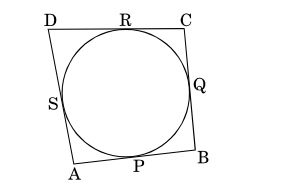
\includegraphics[width=\columnwidth]{figs/circ-1.png}
		
		\caption{}
		\label{fig:circ-1}
	\end{figure}
	\item Draw a pair of tangents to a circle of radius $4 cm$ which are inclined to each other at an angle of 45\degree.	
	\item A point $\vec{T}$ is $13 cm$ away from the centre of a circle. The length of the tangent drawn from $\vec{T}$ to the circle is $12 cm$. Find the radius of the circle.
	\item Two tangents $TP$ and $PQ$ are drawn to a circle with centre $\vec{O}$ from an external point $\vec{T}$. Prove that $\angle PTQ = 2 \angle OPQ$.
	\item $PQ$ is a tangent to a circle with centre $\vec{O}$ at the point $\vec{P}$ on the circle. If $\triangle OPQ$ is an isosceles triangle, then find $\angle OQP$.
	\item Two concentric circles have radii $10 cm$ and $6 cm$. Find the length of the chord of the larger circle which touches the smaller circle.
	\item If tangents $PA$ and $PB$ from an external point $\vec{P}$ to a circle with centre $\vec{O}$ are inclined to each other at an angle of 70\degree, then find $\angle POA$.
	\item $ABC$ is right triangle, right-angled at $\vec{B}$ with $BC = 6 cm$ and $AB = 8 cm$. A circle with centre $\vec{O}$ and radius $r$ cm has been inscribed in $\triangle ABC$ as shown in the figure. Find the value of $r$.
		\begin{figure}[H]
			\centering
			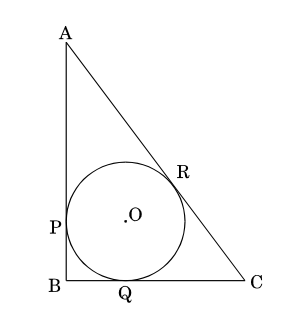
\includegraphics[width=\columnwidth]{figs/circ-2.png}
			\caption{}
			\label{fig:circ-2}
		\end{figure}
	\item Draw a circle of radius $5 cm$. From a point $8 cm$ away from its centre, construct a pair of tangents to the circle.
	\item In the given figure, $PT$ and $PS$ are tangents to a circle with centre $\vec{O}$, from a point $\vec{P}$, such that $PT = 4 cm$ and $\angle TPS = 60$\degree. Find the length of the chord $TS$. Also, find the radius of the circle.
		\begin{figure}[H]
			\centering
			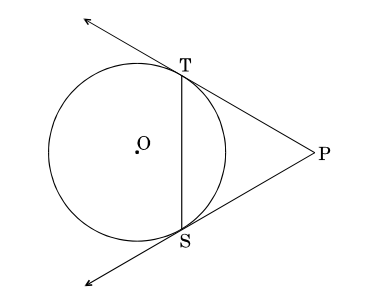
\includegraphics[width=\columnwidth]{figs/circ-3.png}
			\caption{}
			\label{fig:circ-3}
		\end{figure}
	\item \begin{enumerate}[label=(\alph*)]
			\item In a right triangle $ABC$, right-angled at $\vec{B}$, $BC = 6 cm$ and $AB = 8 cm$. A circle is inscribed in the $\triangle ABC$. Find the radius of the incircle.
			\item Two circles touch externally at $\vec{P}$ and $AB$ is a common tangent, touching one circle at $\vec{A}$ and the other at $\vec{B}$. Find the measure of $\angle APB$.
		\end{enumerate}
	\item From an external point $\vec{P}$, tangents $PQ$ and $PR$ are drawn to a circle with centre $\vec{O}$, touching the circle at $\vec{Q}$ and $\vec{R}$. If $\angle QOR = 140$\degree, find the measure of $\angle QPR$.
	\item A circle touches all the sides of a quadrilateral $ABCD$. Prove that $AB + CD = DA + BC$.
	\item Write the steps of construction of a circle of diameter $6 cm$ and drawing of a pair of tangents to the circle from a point $5 cm$ away from the centre.
\end{enumerate}
\end{document}
                                                                                

\chapter{Intersection of Conics}
\section{2022}
\begin{enumerate}[label=\thesection.\arabic*.,ref=\thesection.\theenumi]
\numberwithin{equation}{enumi}
\numberwithin{figure}{enumi}
\numberwithin{table}{enumi}
\item Using integration, find the area of the region enclosed by the curve $ y=x^2 $, the x-axis and the ordinates $x=-2$ \text { and } $x=1$.

\item Using integration, find the area of the region enclosed by line $y=\sqrt{3}x$ semi-circle $y=\sqrt{4-x^2}$ and x-axis in first quadrant.

\item Using integration, find the area of the smaller region enclosed by the curve ${4x^2 + 4y^2} = 9$ and the line $2x + 2y =3$.

\item If the area of the regin bounded by the curve $y^2 = 4ax$ and the line $x = 4a$ is $\dfrac{256}{3}$\hspace{0.2cm} sq. units, then using integration, find the value of a, where $a>0$.

\item Find the area of the region enclosed by the curves $y^2=x$, $x=\dfrac{1}{4}$,  $y=0$ and $x=1$, using integration.

\item If the area of the region bounded bythe line $y=mx$ and the curve $x^2=y$ is $\dfrac{32}{3}$\hspace{0.2cm}sq. units, then find the positive value of m, using integration.

\item If the area between the curves $x = y^2$ and $x = 4$ is divided into two equal parts by the line $x = a$, then find the value of a, using integration.

\item Find the area bounded by the ellipse $x^2+4y^2=16$ and the ordinates $x=0$ and $x=2$, using integration.

\item Find the area of the region $\{(x,y) : x^2 \leq y \leq x\}$, using integration

\end{enumerate}

\section{2021}
\subsection{12}
  \begin{enumerate}
        
\item The point at which the normal to the curve 
\begin{align}
    y = x+\frac{1}{x}, x>0 
\end{align}
 is perpendicular to the line
 \begin{align}
     3x-4y-7 = 0 
 \end{align}
\begin{enumerate}
    \item $\brak{2,\frac{5}{2}}$   \item $\brak{\pm2,\frac{5}{2}}$  

         \item $\brak{-\frac{1}{2},\frac{5}{2}}$    \item $\brak{\frac{1}{2},\frac{5}{2}}$
\end{enumerate}
         
         \item The points on the curve
         \begin{align}
             \frac{x^2}{9} +\frac{y^2}{16} = 1
         \end{align}
         at which the tangents are parallel to $y$-axis are:
         \begin{enumerate}
             \item $\brak{0,\pm4}$   \item $\brak{\pm4,0}$  

         \item  $\brak{\pm3,0}$   \item $\brak{0,\pm3}$
         \end{enumerate}
           
         \item For which value of m is the line
         \begin{align}
            y = mx + 1 
         \end{align}a tangent to the curve 
        \begin{align}
            y^2 = 4x 
        \end{align}
        \begin{enumerate}
            \item  $\frac{1}{2}$  \item $1$

         \item 2  \item 3
        \end{enumerate}
    \end{enumerate}


\chapter{Probability}
\section{2021}
\subsection{10}

\begin{enumerate}
\item During the lockdown period,many families got bored of watching TV all the time.Out of these families, one family of 6 members decided to play a card game.17 cards numbered 1,2,3,4,..,17 are put in a box and mixed thoroughly.One card is drawn by one member at random and other family members bet for the chances of drawing the number either prime,odd or even etc.
\begin{figure}[H]
\centering
	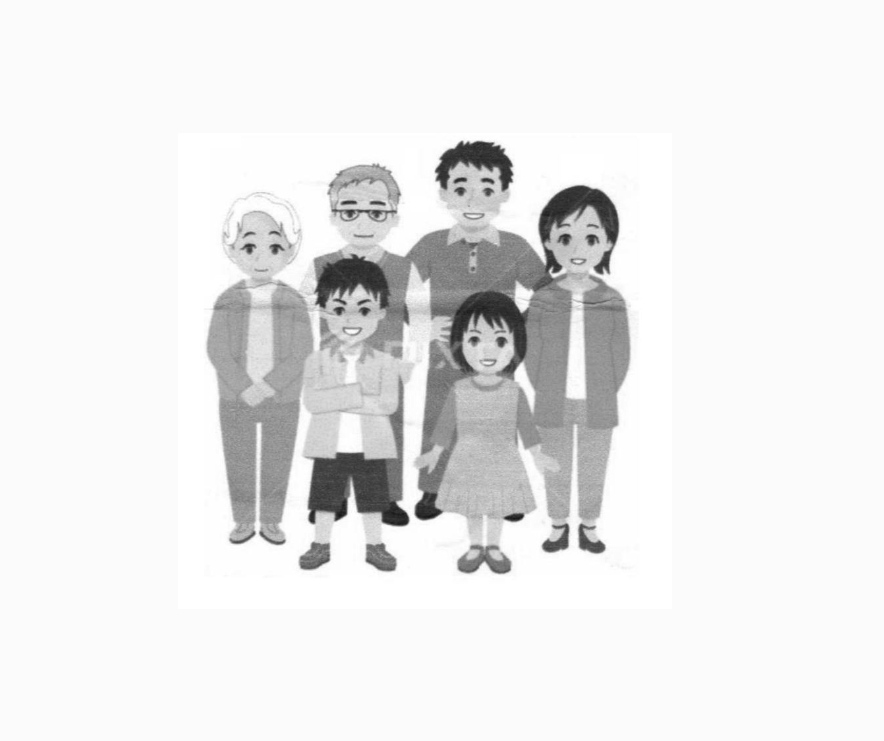
\includegraphics[width=\columnwidth]{figs/satish.jpg}                                                                                              
\caption{Family of six}
\label{fig:satish.jpg}                                                                                                                      \end{figure}
Based on the above,answer the following questions:
\begin{enumerate}                                                                                                                                       \item The first member of the family draws a card at random and another member bets that it is an even prime number.What is the probability of his winning the bet?                                                                                                                           \begin{enumerate}
        \item $\frac{2}{17}$
        \item $\frac{3}{17}$
        \item $\frac{1}{17}$
        \item $\frac{4}{17}$
\end{enumerate}
       \item The second member of the family draws a card at random and some other
member bets that it is an even number. What is the probability of his winning
the bet ?
\begin{enumerate}
        \item $\frac{7}{17}$
        \item $\frac{8}{17}$
        \item $\frac{9}{17}$
        \item $\frac{10}{17}$
\end{enumerate}
      \item What is the probability that the number on the card drawn at random is
divisible by 5 ?
\begin{enumerate}
        \item $\frac{5}{17}$
        \item $\frac{4}{17}$
        \item $\frac{3}{17}$
        \item $\frac{2}{17}$
\end{enumerate}
      \item What is the probability that the number on the card drawn at random is a
multiple of 3 ?
\begin{enumerate}
        \item $\frac{5}{17}$
        \item $\frac{6}{17}$
        \item $\frac{7}{17}$
        \item $\frac{8}{17}$
\end{enumerate}   
\end{enumerate}                                                                                                                                       
\item 
\item Two different coins are tossed simultaneously. Write all the possible outcomes.                                                                   
\item A die is thrown once. Write the probability of getting a number less than $7$.

\item  If the probability of occurrence of event E,\pr{E}=0.99, what is the probability of non-occurrence of the event E,\pr {not E}?                   \item \begin{enumerate}
\item A bag contains 5 white balls and 7 red balls.A ball is drawn at random from the bag.What is the probability that it is either a white or a red ball?
\item Two coins are tossed together once.What is the probability of getting at least one head?
\end{enumerate}
\item Cards marked with numbers $1$,$2$,$3$,$4$, ..., $100$ are placed in a bag and mixed together throughly. A card is randomly drawn from the bag.Find the probability that the numbers on the card is                             \begin{enumerate}                                                                                                                     \item an even number,
\item a $2$-digit number,
\item a perfect square.                                         
\end{enumerate}
\item \begin{enumerate}
\item How many outcomes are possible when three dice are thrown together?
\item if \pr{E}=0.015, then find \pr{not E}.
\end{enumerate}
\item  During summer break, Harish wanted to play with his friends but it was too hot outside, so he decided to play some indoor game with his friends. He collects $20$ identical Icards and writes the numbers $1$ to $20$ on them (one number on one card). He puts them in a box. He and his friends make a bet for the chances of drawing various cards out of the box. Ench was given a chance to tell the probability of picking one card out of the box.

Based on the above,answer the following questions:
\begin{enumerate}                                                                                                                                 \item The probability that the number on the card drawn is an odd prime number,is
\begin{enumerate}                           

          \item $\frac{3}{5}$
          \item $\frac{2}{5}$
          \item $\frac{9}{20}$                      
          \item $\frac{7}{20}$                                               \end{enumerate}
\item The probability that the number on the card drawn is a composite number is
\begin{enumerate}
        \item $\frac{11}{20}$                     
	\item $\frac{3}{5}$                       
	\item $\frac{4}{5}$                     
	\item $\frac{1}{2}$
\end{enumerate}
\item The probability that the number on the card drawn is a multiple of $3$,$6$ and $9$ is
\begin{enumerate}               
	\item $\frac{1}{20}$                      
	\item $\frac{1}{20}$                      
	\item $\frac{3}{20}$                      
	\item $0$
\end{enumerate}
\item The probability that the number on the card drawn is a multiple of $3$ and $7$is
\begin{enumerate}                 
	\item $\frac{3}{10}$                      
	\item $\frac{1}{10}$                      
	\item $0$
        \item $\frac{2}{5}$               
\end{enumerate}                                                              \item If all cards having odd numbers written on them are removed from the box and then one card is drawn from the remaining cards, the probability of getting a card having a prime number is
\begin{enumerate}                
	\item $\frac{1}{20}$
	\item $\frac{1}{10}$                      
        \item $0$ 
        \item $\frac{1}{5}$               
\end{enumerate}
\end{enumerate}
\item \begin{enumerate}
\item In a single throw of a pair of dice,find the probability that both dice have the same number.
\item A card is drawn from a well-shuffled pack of $52$ cards.Find the probability that it is not an ace.
\end{enumerate}
\end{enumerate}

\subsection{12}
\documentclass{article}
\usepackage{siunitx}
\usepackage{setspace}
\usepackage{gensymb}          
\usepackage{xcolor}
\usepackage{caption}
%\usepackage{subcaption}
%\doublespacing               
\singlespacing   
\usepackage[none]{hyphenat}   
\usepackage{amssymb} 
%\usepackage{relsize} 
\usepackage[cmex10]{amsmath}  
\usepackage{mathtools}      
\usepackage{amsmath}   
\usepackage{commath}  
%\usepackage{amsthm}    
%\interdisplaylinepenalty=2500 
%\savesymbol{iint}   
%\usepackage{txfonts}
%\restoresymbol{TXF}{iint}  
%\usepackage{wasysym}    
\usepackage{amsthm}   
\usepackage{mathrsfs}
\usepackage{txfonts}
\let\vec\mathbf{}
%\usepackage{stfloats}
\usepackage{float}
\usepackage{cite}
\usepackage{cases}
\usepackage{subfig}
%\usepackage{xtab}
\usepackage{longtable}
\usepackage{multirow}
%\usepackage{algorithm}
\usepackage{amssymb}
%\usepackage{algpseudocode}
\usepackage{enumitem}
\usepackage{mathtools}
%\usepackage{eenrc}
%\usepackage[framemethod=tikz]{mdframed}
\usepackage{listings}
\usepackage{listings}         
\usepackage[latin1]{inputenc}   
%% \usepackage{color}        
%% \usepackage{lscape}       
\usepackage{titling}                 
%\usepackage{fulbigskip}   
\usepackage{tikz}      
\usepackage{graphicx}
\graphicspath{{/Internal storage/Download/FWC
}}
\usepackage{atbegshi}
%http://ctan.org/pkg/atbegshi
\AtBeginDocument{\AtBeginShipoutNext{\AtBeginShipoutDiscard}}
%
\begin{document}
\begin{center}
\title{\textbf{CBSE - 12} \\ {PROBABILITY}}

\date{}
\maketitle
\end{center}
\begin{enumerate}
    \item The probability of solving a specific question independently by $A$ and $B$ are $\frac{1}{3}$ and $\frac{1}{5}$ respectively.If both try to solve the question independently, the probability that the question is solved is
    \begin{enumerate}
        \item $\frac{7}{15}$
        \item $\frac{8}{15}$
        \item $\frac{2}{15}$
        \item $\frac{14}{15}$
    \end{enumerate}
   
    \item From a pack of 52 cards, 3 cards are drawn at random (without replacement).The probability that they are two red cards and one black card is$\underline{\hspace{2cm}}$.
    \item A bag contains 19 tickets, numbered 1 to 19. A ticket is drawn at random and then another ticket is drawn without replacing the first one in the bag. Find the probability distribution of the number of even numbers on the ticket.
   
    \item Find the probability distribution of the number of successes in two tosses of a die, when a success is defined as "number greater than 5".
    \item A bag contains 5 red and 4 black balls, a second bag contains 3 red and 6 black balls. One of the two bags is selected at random and two balls are drawn at random (without replacement), both of which are found to be red. Find the probability that these two balls are drawn from the second bag.
   
    
    \item An unbiased die is thrown. What is the probability of getting an odd number or a multiple of 3 ?\begin{enumerate}
        \item $\frac{3}{4}$
        \item $\frac{1}{2}$
        \item $\frac{2}{3}$
        \item $\frac{1}{3}$
    \end{enumerate}
    \item A card is drawn from an ordinary pack of 52 cards and a gambler bets that it 
is a heart or a king card. What are the odds against his winning this bet ?
\begin{enumerate}
    \item 4 : 9
    \item 1 : 4
    \item 4 : 1
    \item 9 : 4
\end{enumerate}
\item In a lottery of 25 tickets, numbered 1 to 25, two tickets are drawn simultaneously. Find the probability that none of the tickets has prime number.
\item If $E_1$ and $E_2$ are two events, where $E_1$ is a subset of $E_2$, then evaluate $P(E_2 \mid E_1)$.
\item Two dice are thrown simultaneously. Find the probability of getting a multiple of 3 on one dice and a multiple of 2 on the other dice.

 \item An urn contains 4 white, 7 green and 9 blue balls. If two balls are drawn at random, find the probability that the drawn balls are of the same colour. 
\end{enumerate}

\end{document}

\section{2023}
\subsection{10}
\begin{enumerate}
	\item Probability of happining of an event is denoted by $p$ and probability of non-happening of the event is denoted by $q$. Relation between $p$ and $q$ is
                        \begin{enumerate}
                                \item $p$+$q$=1
                                \item $p$=1, $q$=1
                                \item $p$=$q$-1
                                \item $p$+$q$+1=0
                        \end{enumerate}
			
        \item A girl calculates that the probability of her winning the first prize in a lottery is 0.08. If 6000 tickets are sold, how many tickets has she bought ?
                        \begin{enumerate}
                                \item  40
                                \item  240
                                \item  480
                                \item  750

                        \end{enumerate}
        \item In a group of 20 people, 5 can't swim. If one person is selected at random, then the probability that he/sh can swim, is
                        \begin{enumerate}
                                \item $ \frac {3} {4} $
                                \item $ \frac {1} {3} $
                                \item 1
                                \item $ \frac {1} {4} $
                        \end{enumerate}
        \item A bag contain 4 red, 3 blue and 2 yellow balls. One ball is drawn at random from the bag. Find the probability that drawn ball is
                \begin{enumerate}
                                        \item red
                                        \item yellow
                \end{enumerate}
        \item A bag contain 100 cards numbered 1 to 100.Acard is drawn at random from the b. What is the probability that the number on the card is a perfect cube ?
                        \begin{enumerate}
                                \item $ \frac {1} {20} $
                                \item $ \frac {3} {50} $
                                \item $ \frac {1} {25} $
                                \item $ \frac {7} {100} $
                        \end{enumerate}
        \item If three coins are tossed simultaneously, what is the probability of getting a most one trail ?
                        \begin{enumerate}
                                \item $ \frac {3} {8} $
                                \item $ \frac {4} {8} $
                                \item $ \frac {5} {8} $
                                \item $ \frac {7} {8} $
                        \end{enumerate}
        \item Two dics are thrown together. The probability of getting the difference of numbers on their upper faces equals to 3 is :
                        \begin{enumerate}
                                \item $ \frac {1} {9} $
                                \item $ \frac {2} {9} $
                                \item $ \frac {1} {6} $
                                \item $ \frac {1} {12} $
                        \end{enumerate}
        \item A card is drawn at random from a well-shuffled pack of 52 cards. The probability that the card drawn is not an ace is :

                        \begin{enumerate}
                                \item $ \frac {1} {13} $
                                \item $ \frac {9} {13} $
                                \item $ \frac {4} {13} $
                                \item $ \frac {12} {13} $
                        \end{enumerate}
        \item \textbf{Assertion (A) : } The probability that a leap year has 53 Students is $ \frac {2} {7} $.\\
                \textbf{Reason (R) : } The probability that a non-leap year has 53 Sundays is $ \frac {5} {7} $.

                          \begin{enumerate}
                                  \item Both Assertion (A) and Reason (R) are true and Reason (R) is the correct explanation of Assertion (A).
                                  \item Both Assertion (A) and Reason (R) are true and Reason (R) is not the correct explanation of Assertion (A).
                                  \item Assertion (A) is true but Reason (R) is false.
                                  \item Assertion (A) is false but Reason (R) is true.
                          \end{enumerate}


\end{enumerate}

\subsection{12}
\begin{enumerate}[label=\thesection.\arabic*.,ref=\thesection.\theenumi]
\numberwithin{equation}{enumi}
\numberwithin{figure}{enumi}
\numberwithin{table}{enumi}
	
	\item If A and B are two events such that 
		\begin{align}
			\pr{A|B} = 2 \times  \pr{B|A}\pr{A} + \pr{B}  = \frac{2}{3}
		\end{align}then \pr{B}  is equal to
\begin{enumerate}
\item $\frac{2}{9}$
\item $\frac{7}{9}$
\item $\frac{4}{9}$
\item $\frac{5}{9}$
\end{enumerate}

\item
\begin{enumerate}
\item Two balls are drawn at random one by one with replacement from an urn containing equal number of red balls and green balls. Find the probability distribution of number of red balls. Also, find the mean of the random variable.
\item A and B throw a die alternately till one of them gets '6' and wins the game. Find their respective probabilities of winning, if A starts the game first.
\end{enumerate}

\item Recent studies suggest that roughly $12\%$ of the world population is left handed.
	
\begin{figure}[h!]
\centering
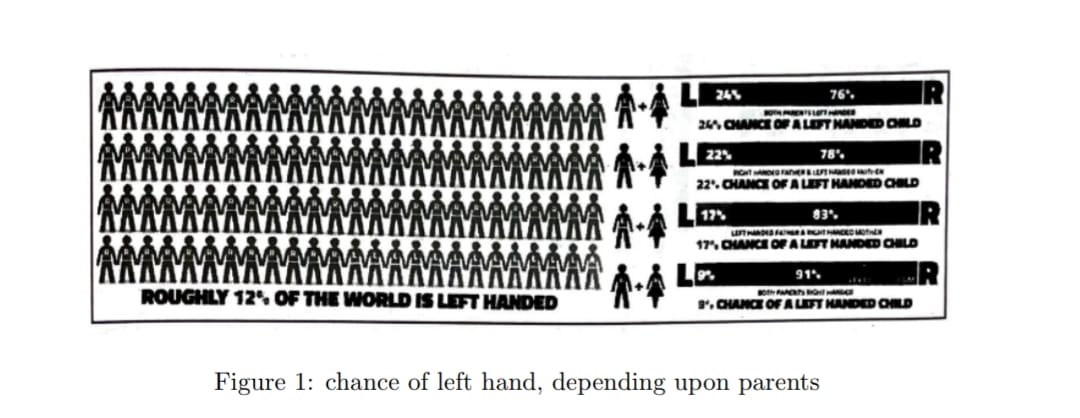
\includegraphics[width=\columnwidth]{figs/left.png}
\caption{chance of left hand, depending upon parents}
\label{fig:left.png}
\end{figure}

Depending upon the parents, the chances of having a left handed child are as follows :\\
\begin{enumerate}
\item   When both father and mother are left handed :
        Chances of left handed child is $24\%$.
\item   When father is right handed and mother is left handed :
        Chances of left handed child is $22\%$.
\item   when father is left handed and mother is right handed :
        Chances of left handed child is $17\%$.
\item   When both father nd mother are right handed :
        Chances of left handed child is $9\%$.
\end{enumerate}
Assuming that $\pr{A}=\pr{B}=\pr{C}=\pr{D}=\frac{1}{4}$ and L denotes the event that child is left handed.
Based on the above information, answer the following questions :\\
\begin{enumerate}
	\item    Find \pr{L|C}
	\item    Find \pr{\overline{L}|A}
	\item    Find \pr{A|L}
\item    Find the probability that a randomly selected child is left handed given that exactly one of the parent is left handed.
\end{enumerate}
\end{enumerate}

\section{2022}
\subsection{12}
\begin{enumerate}[label=\thesection.\arabic*.,ref=\thesection.\theenumi]
\numberwithin{equation}{enumi}
\numberwithin{figure}{enumi}
\numberwithin{table}{enumi}
\item Let A and B be two events such that $P(A) = \frac{5}{8}$, $P(B) = \frac{1}{2}$ and  $P(A|B) = \frac{3}{4}$. Find the value of $P(B|A)$.
\item Two balls are drawn at random from a bag containing 2 red balls and 3 blue balls, without replacement. Let the variables X denotes the number of red balls. Find the probabillity distribution of X.
\item A card from a pack of 52 playing cards is lost. From the remaining cards, 2 cards are drawn at random without replacement, and are found to be both aces. Find the probability that lost card being an ace.
\item Probabilities of A and B solving a specific problem are $\frac{2}{3}$ and $\frac{3}{5},$ respectively. If both of them try independently to solve the problem, then find the probability that the problem is  solved.
\item A pair of dice is thrown. It is given that the sum of numbers  appearing on both dice is an even number. Find the probability that the number apprearing on at least one die is 3.
\item At the start of a cricket match, a coin is tossed and the team winning the toss has the opportunity to choose to bat or bowl. such a coin is unbaised with equal probabilities of getting head and tail \figref{fig:2022/probability/coin1} .
\begin{figure}[!ht]
\centering

\includegraphics[width=\columnwidth]{figs/coin}
\caption{Toss before the match}
\label{fig:2022/probability/coin1}
\end{figure}
\\ Based on the above information, answer the following question:
\begin{enumerate}
\item If such a coin is tossed 2 times, then find the probability distibution of numbers of tails.
\item Find the probability of getting at least one head in three tosses of such a coin.
\end{enumerate}
\item Two cards are drawn successively with replacement from a well shuffled pack of 52 cards. Find the probability distribution of the number of spade cards.
\item A pair of dice is thrown and the sum of the numbers appearing on the dice is observed to be 7. Find the probability that the number 5 has appeared on at least one die.
\item The probability that A hits the target is $\frac{1}{3}$ and the probability that B hits it, is $\frac{2}{5}.$ If both try to hit the target independently, find the probabillity that the target is hit. 
\item A shopkeeper sells three types of flower seeds A$_1$ , A$_1$ , A$_3$. They are sold in the form of a mixture, where the proportions of these seeds are  4 : 4 : 2, respectively. The germinaton rates of the three types of seeds are $45\%,$ $60\%$ and $35\%$ respectively \figref{fig:2022/probability/flowers11}.
\begin{figure}[!ht]
\centering                                  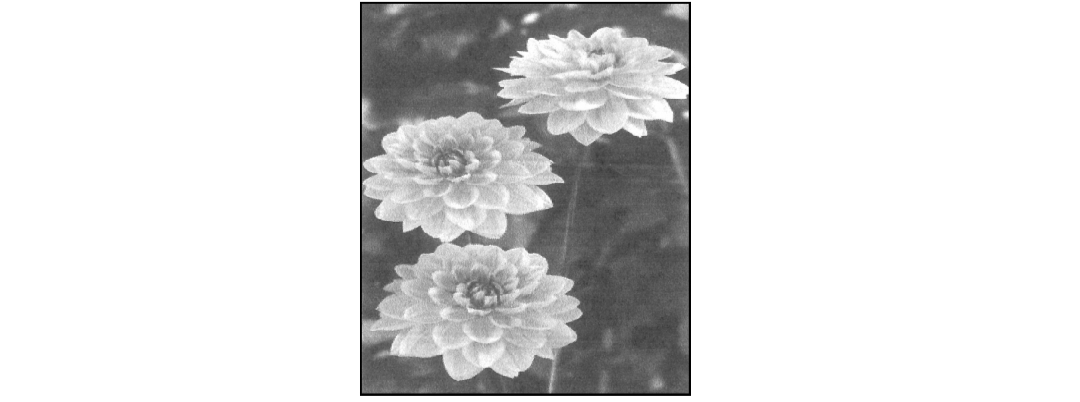
\includegraphics[width=\columnwidth]{figs/flowers}                                     
\caption{Three types of flowers}            
\label{fig:2022/probability/flowers11}                       
\end{figure}
\\ Based on  the above information :
\begin{enumerate}
\item  Calculate the probability that a randomly chosen seed will germinate.
\item  Calculate the probability  that the seed is of type $A_2$, given that a randomly choosen seed germinates.
\end{enumerate}
\item Three friends A, B and C got their photograph clicked. Find the probability that B is standing at the central position, given that A is standing at the left corner.
\item In a game of Archery, each ring of the Archery target is valued. The centremost ring is worth 10 points and rest of the rings are alloted points 9 to 1 in sequential order moving outwards.Archer A is likely to earn 10 points with a probability of 0.8 and Archer B is likely the earn 10 points with a probability of 0.9 \figref{fig:2022/probability/archery3}.
\begin{figure}[!ht]                     
\centering
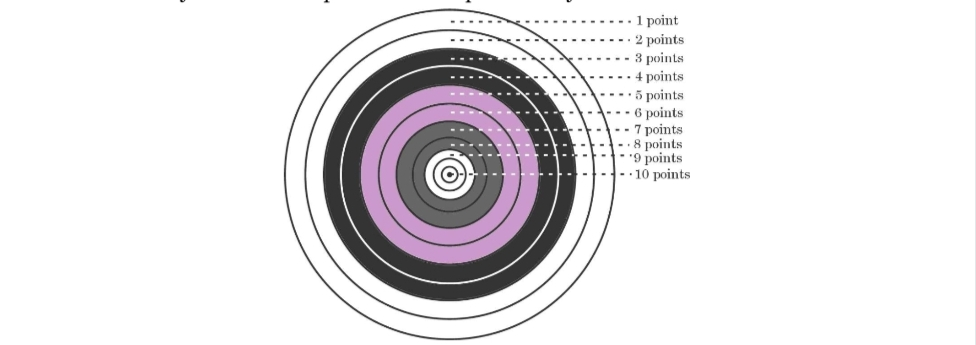
\includegraphics[width=\columnwidth]{figs/archery}
\caption{centermost ring}                   
\label{fig:2022/probability/archery3}                        
\end{figure}
\\ Based on the above innformation, answer the following questions :
\begin{enumerate}
\item exactly one of them earns 10 points .
\item both of them earn 10 point.
\end{enumerate}
\item Event A and B are such that \begin{align} P(A) = \frac{1}{2},  P(B) = \frac{7}{12}\end{align} and \begin{align} P(\bar{A}\cup \bar{B}) = \frac{1}{4} \end{align}
Find whether the events  A and B are independent or not.
\item A box $B_1$ contain 1 white ball  and 3 red balls. Another box $B_2$ contains 2 white balls and 3 red balls. If one ball is drawn at random from each of the boxes $B_1$ and $B_2$, then find the probability that the two balls drawn are of the same colour.
\item Let X be random variable which assumes values $x_1$, $x_2$, $x_3$, $x_4$  such that\begin{align} 2P(X = x_1) = 3P (X = x_2) = P ( X = x_3) = 5P (X = x_4).\end{align}
\\ Find the probability distribution of X.
\item There are two boxes, namely box-I and box-II. Box-I contains  3 red and 6 black balls. Box-II contains 5 red and 5 black balls. One of the two boxes , is selected at random and a ball is drawn at random. The ball drawn is found to be red. Find the probability that this red ball comes out from box-II.
\item In a toss of three different coins, find the probability of comming up of three heads, if it is known that at least one head comes up.
\item A laboratory blood text is $98\%$ effective  in detecting a certain disease when it is fact, present. However, the text also yeilds a false positive result for $0.4\%$ of the healthy person tested. From a large population, it is given that $0.2\%$ of the population actually has the diseases.
\\Based on the above, answer the following questtion : 
\begin{enumerate}
\item one person, from the population, is taken at random and given the test. Find the probabiliy of his getting a positive test result.
\item what is the probability that the person actually has the disease, given that his test result is positive ?
\end{enumerate}
\item Two cards are drawn from a well-shuffled pack of playing cards one-by-one with replacement. The probability that the first card is a king and the second card is a queen is 
\begin{enumerate}
\item $\frac{1}{13} + \frac{1}{13}$
\item $ \frac{1}{13} \times \frac{4}{51}$
\item $\frac{4}{52} \times \frac{3}{51}$
\item $\frac{1}{13} \times \frac{1}{13}$
\end{enumerate}
\item For two events A and B if P(A) = $\frac{4}{10}, P{B} = \frac{8}{10}$ and $P(B|A)$ = $\frac{6}{10}$ then find $P( A \cup B).$
\item Bag I contain 4 red and 3 black balls. Bag II contains 3 red and 5 black balls. One of two bags is selected at random and a ball is drawn from the bag, which if found to be red. Find the probability that the ball is drawn from bag II.
\item Two cards are drawn successively without replacement from a well-shuffled pack of 52 cards. Find the probability distribution of the number of aces and hence find its mean.
\item The probability of solving a specific question independently by A and B are $\frac{1}{3}$ and $\frac{1}{5}$ respectively . If both try to solve the question independently, the probability that the question is solved is 
\begin{enumerate}
\item $\frac{7}{15}$
\item $\frac{8}{15}$
\item $\frac{2}{15}$
\item $\frac{14}{15}$
\end{enumerate}
\item A card is picked at random from a pack of 52 playing cards. Given that the picked up card is a queen, the probability of it being a queen of spades is \underline{\hspace{1cm}}.
\item A bag contains 19 tickets, numbered 1 to 19. A ticket is drawn at random and then another ticket is drawn without replacing the first one in the bag. Find the probability distribution of the number of even numbers on the ticket.
\item Find the probability distribution of the numbers of successes in two tosses of a die, when a success is defined as number greater than 5.
\item Ten cartoons are taken at random from an automatic packing machine. The mean net weight of the ten carton is 11.8 kg and standard deviation is 0.15 kg. Does the sample mean differ significantly from the intended mean of 12 kg ?
[Given that for d.f. = 9, $t_{0.05}$ = 2.26]
\item A Coin is tossed twice. The following table\ref{tab: Number of tails} shows the probability distribution of numbers of tails:
\begin{table}[!ht]
%%%%%%%%%%%%%%%%%%%%%%%%%%%%%%%%%%%%%%%%%%%%%%%%%%%%%%%%%%%%%%%%%%%%%%
%%                                                                  %%
%%  This is the header of a LaTeX2e file exported from Gnumeric.    %%
%%                                                                  %%
%%  This file can be compiled as it stands or included in another   %%
%%  LaTeX document. The table is based on the longtable package so  %%
%%  the longtable options (headers, footers...) can be set in the   %%
%%  preamble section below (see PRAMBLE).                           %%
%%                                                                  %%
%%  To include the file in another, the following two lines must be %%
%%  in the including file:                                          %%
%%        \def\inputGnumericTable{}                                 %%
%%  at the beginning of the file and:                               %%
%%        \input{name-of-this-file.tex}                             %%
%%  where the table is to be placed. Note also that the including   %%
%%  file must use the following packages for the table to be        %%
%%  rendered correctly:                                             %%
%%    \usepackage[latin1]{inputenc}                                 %%
%%    \usepackage{color}                                            %%
%%    \usepackage{array}                                            %%
%%    \usepackage{longtable}                                        %%
%%    \usepackage{calc}                                             %%
%%    \usepackage{multirow}                                         %%
%%    \usepackage{hhline}                                           %%
%%    \usepackage{ifthen}                                           %%
%%  optionally (for landscape tables embedded in another document): %%
%%    \usepackage{lscape}                                           %%
%%                                                                  %%
%%%%%%%%%%%%%%%%%%%%%%%%%%%%%%%%%%%%%%%%%%%%%%%%%%%%%%%%%%%%%%%%%%%%%%



%%  This section checks if we are begin input into another file or  %%
%%  the file will be compiled alone. First use a macro taken from   %%
%%  the TeXbook ex 7.7 (suggestion of Han-Wen Nienhuys).            %%
\def\ifundefined#1{\expandafter\ifx\csname#1\endcsname\relax}


%%  Check for the \def token for inputed files. If it is not        %%
%%  defined, the file will be processed as a standalone and the     %%
%%  preamble will be used.                                          %%
\ifundefined{inputGnumericTable}

%%  We must be able to close or not the document at the end.        %%
	\def\gnumericTableEnd{\end{document}}


%%%%%%%%%%%%%%%%%%%%%%%%%%%%%%%%%%%%%%%%%%%%%%%%%%%%%%%%%%%%%%%%%%%%%%
%%                                                                  %%
%%  This is the PREAMBLE. Change these values to get the right      %%
%%  paper size and other niceties.                                  %%
%%                                                                  %%
%%%%%%%%%%%%%%%%%%%%%%%%%%%%%%%%%%%%%%%%%%%%%%%%%%%%%%%%%%%%%%%%%%%%%%

	\documentclass[12pt%
			  %,landscape%
                    ]{report}
       \usepackage[latin1]{inputenc}
       \usepackage{fullpage}
       \usepackage{color}
       \usepackage{array}
       \usepackage{longtable}
       \usepackage{calc}
       \usepackage{multirow}
       \usepackage{hhline}
       \usepackage{ifthen}

	\begin{document}


%%  End of the preamble for the standalone. The next section is for %%
%%  documents which are included into other LaTeX2e files.          %%
\else

%%  We are not a stand alone document. For a regular table, we will %%
%%  have no preamble and only define the closing to mean nothing.   %%
    \def\gnumericTableEnd{}

%%  If we want landscape mode in an embedded document, comment out  %%
%%  the line above and uncomment the two below. The table will      %%
%%  begin on a new page and run in landscape mode.                  %%
%       \def\gnumericTableEnd{\end{landscape}}
%       \begin{landscape}


%%  End of the else clause for this file being \input.              %%
\fi

%%%%%%%%%%%%%%%%%%%%%%%%%%%%%%%%%%%%%%%%%%%%%%%%%%%%%%%%%%%%%%%%%%%%%%
%%                                                                  %%
%%  The rest is the gnumeric table, except for the closing          %%
%%  statement. Changes below will alter the table's appearance.     %%
%%                                                                  %%
%%%%%%%%%%%%%%%%%%%%%%%%%%%%%%%%%%%%%%%%%%%%%%%%%%%%%%%%%%%%%%%%%%%%%%

\providecommand{\gnumericmathit}[1]{#1} 
%%  Uncomment the next line if you would like your numbers to be in %%
%%  italics if they are italizised in the gnumeric table.           %%
%\renewcommand{\gnumericmathit}[1]{\mathit{#1}}
\providecommand{\gnumericPB}[1]%
{\let\gnumericTemp=\\#1\let\\=\gnumericTemp\hspace{0pt}}
 \ifundefined{gnumericTableWidthDefined}
        \newlength{\gnumericTableWidth}
        \newlength{\gnumericTableWidthComplete}
        \newlength{\gnumericMultiRowLength}
        \global\def\gnumericTableWidthDefined{}
 \fi
%% The following setting protects this code from babel shorthands.  %%
 \ifthenelse{\isundefined{\languageshorthands}}{}{\languageshorthands{english}}
%%  The default table format retains the relative column widths of  %%
%%  gnumeric. They can easily be changed to c, r or l. In that case %%
%%  you may want to comment out the next line and uncomment the one %%
%%  thereafter                                                      %%
\providecommand\gnumbox{\makebox[0pt]}
%%\providecommand\gnumbox[1][]{\makebox}

%% to adjust positions in multirow situations                       %%
\setlength{\bigstrutjot}{\jot}
\setlength{\extrarowheight}{\doublerulesep}

%%  The \setlongtables command keeps column widths the same across  %%
%%  pages. Simply comment out next line for varying column widths.  %%
\setlongtables

\setlength\gnumericTableWidth{%
	53pt+%
	53pt+%
	53pt+%
	53pt+%
0pt}
\def\gumericNumCols{4}
\setlength\gnumericTableWidthComplete{\gnumericTableWidth+%
         \tabcolsep*\gumericNumCols*2+\arrayrulewidth*\gumericNumCols}
\ifthenelse{\lengthtest{\gnumericTableWidthComplete > \linewidth}}%
         {\def\gnumericScale{1*\ratio{\linewidth-%
                        \tabcolsep*\gumericNumCols*2-%
                        \arrayrulewidth*\gumericNumCols}%
{\gnumericTableWidth}}}%
{\def\gnumericScale{1}}

%%%%%%%%%%%%%%%%%%%%%%%%%%%%%%%%%%%%%%%%%%%%%%%%%%%%%%%%%%%%%%%%%%%%%%
%%                                                                  %%
%% The following are the widths of the various columns. We are      %%
%% defining them here because then they are easier to change.       %%
%% Depending on the cell formats we may use them more than once.    %%
%%                                                                  %%
%%%%%%%%%%%%%%%%%%%%%%%%%%%%%%%%%%%%%%%%%%%%%%%%%%%%%%%%%%%%%%%%%%%%%%

\ifthenelse{\isundefined{\gnumericColA}}{\newlength{\gnumericColA}}{}\settowidth{\gnumericColA}{\begin{tabular}{@{}p{53pt*\gnumericScale}@{}}x\end{tabular}}
\ifthenelse{\isundefined{\gnumericColB}}{\newlength{\gnumericColB}}{}\settowidth{\gnumericColB}{\begin{tabular}{@{}p{53pt*\gnumericScale}@{}}x\end{tabular}}
\ifthenelse{\isundefined{\gnumericColC}}{\newlength{\gnumericColC}}{}\settowidth{\gnumericColC}{\begin{tabular}{@{}p{53pt*\gnumericScale}@{}}x\end{tabular}}
\ifthenelse{\isundefined{\gnumericColD}}{\newlength{\gnumericColD}}{}\settowidth{\gnumericColD}{\begin{tabular}{@{}p{53pt*\gnumericScale}@{}}x\end{tabular}}

\begin{longtable}[c]{%
	b{\gnumericColA}%
	b{\gnumericColB}%
	b{\gnumericColC}%
	b{\gnumericColD}%
	}

%%%%%%%%%%%%%%%%%%%%%%%%%%%%%%%%%%%%%%%%%%%%%%%%%%%%%%%%%%%%%%%%%%%%%%
%%  The longtable options. (Caption, headers... see Goosens, p.124) %%
%	\caption{The Table Caption.}             \\	%
% \hline	% Across the top of the table.
%%  The rest of these options are table rows which are placed on    %%
%%  the first, last or every page. Use \multicolumn if you want.    %%

%%  Header for the first page.                                      %%
%	\multicolumn{4}{c}{The First Header} \\ \hline 
%	\multicolumn{1}{c}{colTag}	%Column 1
%	&\multicolumn{1}{c}{colTag}	%Column 2
%	&\multicolumn{1}{c}{colTag}	%Column 3
%	&\multicolumn{1}{c}{colTag}	\\ \hline %Last column
%	\endfirsthead

%%  The running header definition.                                  %%
%	\hline
%	\multicolumn{4}{l}{\ldots\small\slshape continued} \\ \hline
%	\multicolumn{1}{c}{colTag}	%Column 1
%	&\multicolumn{1}{c}{colTag}	%Column 2
%	&\multicolumn{1}{c}{colTag}	%Column 3
%	&\multicolumn{1}{c}{colTag}	\\ \hline %Last column
%	\endhead

%%  The running footer definition.                                  %%
%	\hline
%	\multicolumn{4}{r}{\small\slshape continued\ldots} \\
%	\endfoot

%%  The ending footer definition.                                   %%
%	\multicolumn{4}{c}{That's all folks} \\ \hline 
%	\endlastfoot
%%%%%%%%%%%%%%%%%%%%%%%%%%%%%%%%%%%%%%%%%%%%%%%%%%%%%%%%%%%%%%%%%%%%%%

\hhline{|-|-|-|-}
	 \multicolumn{1}{|p{\gnumericColA}|}%
	{\gnumericPB{\centering}\gnumbox{X}}
	&\multicolumn{1}{p{\gnumericColB}|}%
	{\gnumericPB{\centering}\gnumbox{0}}
	&\multicolumn{1}{p{\gnumericColC}|}%
	{\gnumericPB{\centering}\gnumbox{1}}
	&\multicolumn{1}{p{\gnumericColD}|}%
	{\gnumericPB{\centering}\gnumbox{2}}
\\
\hhline{|----|}
	 \multicolumn{1}{|p{\gnumericColA}|}%
	{\gnumericPB{\centering}\gnumbox{P(X)}}
	&\multicolumn{1}{p{\gnumericColB}|}%
	{\gnumericPB{\centering}\gnumbox{K}}
	&\multicolumn{1}{p{\gnumericColC}|}%
	{\gnumericPB{\centering}\gnumbox{6K}}
	&\multicolumn{1}{p{\gnumericColD}|}%
	{\gnumericPB{\centering}\gnumbox{9K}}
\\
\hhline{|-|-|-|-|}
\end{longtable}

\ifthenelse{\isundefined{\languageshorthands}}{}{\languageshorthands{\languagename}}
\gnumericTableEnd
	
\caption{Table shows the probability distribution of numbers of tails \label{tab: Number of tails}}
\end{table}
\begin{enumerate}
\item Find the value of $K$.
\item Is the coin tossed biased or unbaised?
Justify your answer.
\end{enumerate}
\item If X is a random variable with probability distribution as given below \ref{tab:probability distribution}:
\begin{table}[!ht]
%%%%%%%%%%%%%%%%%%%%%%%%%%%%%%%%%%%%%%%%%%%%%%%%%%%%%%%%%%%%%%%%%%%%%%
%%                                                                  %%
%%  This is the header of a LaTeX2e file exported from Gnumeric.    %%
%%                                                                  %%
%%  This file can be compiled as it stands or included in another   %%
%%  LaTeX document. The table is based on the longtable package so  %%
%%  the longtable options (headers, footers...) can be set in the   %%
%%  preamble section below (see PRAMBLE).                           %%
%%                                                                  %%
%%  To include the file in another, the following two lines must be %%
%%  in the including file:                                          %%
%%        \def\inputGnumericTable{}                                 %%
%%  at the beginning of the file and:                               %%
%%        \input{name-of-this-file.tex}                             %%
%%  where the table is to be placed. Note also that the including   %%
%%  file must use the following packages for the table to be        %%
%%  rendered correctly:                                             %%
%%    \usepackage[latin1]{inputenc}                                 %%
%%    \usepackage{color}                                            %%
%%    \usepackage{array}                                            %%
%%    \usepackage{longtable}                                        %%
%%    \usepackage{calc}                                             %%
%%    \usepackage{multirow}                                         %%
%%    \usepackage{hhline}                                           %%
%%    \usepackage{ifthen}                                           %%
%%  optionally (for landscape tables embedded in another document): %%
%%    \usepackage{lscape}                                           %%
%%                                                                  %%
%%%%%%%%%%%%%%%%%%%%%%%%%%%%%%%%%%%%%%%%%%%%%%%%%%%%%%%%%%%%%%%%%%%%%%



%%  This section checks if we are begin input into another file or  %%
%%  the file will be compiled alone. First use a macro taken from   %%
%%  the TeXbook ex 7.7 (suggestion of Han-Wen Nienhuys).            %%
\def\ifundefined#1{\expandafter\ifx\csname#1\endcsname\relax}


%%  Check for the \def token for inputed files. If it is not        %%
%%  defined, the file will be processed as a standalone and the     %%
%%  preamble will be used.                                          %%
\ifundefined{inputGnumericTable}

%%  We must be able to close or not the document at the end.        %%
	\def\gnumericTableEnd{\end{document}}


%%%%%%%%%%%%%%%%%%%%%%%%%%%%%%%%%%%%%%%%%%%%%%%%%%%%%%%%%%%%%%%%%%%%%%
%%                                                                  %%
%%  This is the PREAMBLE. Change these values to get the right      %%
%%  paper size and other niceties.                                  %%
%%                                                                  %%
%%%%%%%%%%%%%%%%%%%%%%%%%%%%%%%%%%%%%%%%%%%%%%%%%%%%%%%%%%%%%%%%%%%%%%

	\documentclass[12pt%
			  %,landscape%
                    ]{report}
       \usepackage[latin1]{inputenc}
       \usepackage{fullpage}
       \usepackage{color}
       \usepackage{array}
       \usepackage{longtable}
       \usepackage{calc}
       \usepackage{multirow}
       \usepackage{hhline}
       \usepackage{ifthen}

	\begin{document}


%%  End of the preamble for the standalone. The next section is for %%
%%  documents which are included into other LaTeX2e files.          %%
\else

%%  We are not a stand alone document. For a regular table, we will %%
%%  have no preamble and only define the closing to mean nothing.   %%
    \def\gnumericTableEnd{}

%%  If we want landscape mode in an embedded document, comment out  %%
%%  the line above and uncomment the two below. The table will      %%
%%  begin on a new page and run in landscape mode.                  %%
%       \def\gnumericTableEnd{\end{landscape}}
%       \begin{landscape}


%%  End of the else clause for this file being \input.              %%
\fi

%%%%%%%%%%%%%%%%%%%%%%%%%%%%%%%%%%%%%%%%%%%%%%%%%%%%%%%%%%%%%%%%%%%%%%
%%                                                                  %%
%%  The rest is the gnumeric table, except for the closing          %%
%%  statement. Changes below will alter the table's appearance.     %%
%%                                                                  %%
%%%%%%%%%%%%%%%%%%%%%%%%%%%%%%%%%%%%%%%%%%%%%%%%%%%%%%%%%%%%%%%%%%%%%%

\providecommand{\gnumericmathit}[1]{#1} 
%%  Uncomment the next line if you would like your numbers to be in %%
%%  italics if they are italizised in the gnumeric table.           %%
%\renewcommand{\gnumericmathit}[1]{\mathit{#1}}
\providecommand{\gnumericPB}[1]%
{\let\gnumericTemp=\\#1\let\\=\gnumericTemp\hspace{0pt}}
 \ifundefined{gnumericTableWidthDefined}
        \newlength{\gnumericTableWidth}
        \newlength{\gnumericTableWidthComplete}
        \newlength{\gnumericMultiRowLength}
        \global\def\gnumericTableWidthDefined{}
 \fi
%% The following setting protects this code from babel shorthands.  %%
 \ifthenelse{\isundefined{\languageshorthands}}{}{\languageshorthands{english}}
%%  The default table format retains the relative column widths of  %%
%%  gnumeric. They can easily be changed to c, r or l. In that case %%
%%  you may want to comment out the next line and uncomment the one %%
%%  thereafter                                                      %%
\providecommand\gnumbox{\makebox[0pt]}
%%\providecommand\gnumbox[1][]{\makebox}

%% to adjust positions in multirow situations                       %%
\setlength{\bigstrutjot}{\jot}
\setlength{\extrarowheight}{\doublerulesep}

%%  The \setlongtables command keeps column widths the same across  %%
%%  pages. Simply comment out next line for varying column widths.  %%
\setlongtables

\setlength\gnumericTableWidth{%
	53pt+%
	53pt+%
	53pt+%
	53pt+%
0pt}
\def\gumericNumCols{4}
\setlength\gnumericTableWidthComplete{\gnumericTableWidth+%
         \tabcolsep*\gumericNumCols*2+\arrayrulewidth*\gumericNumCols}
\ifthenelse{\lengthtest{\gnumericTableWidthComplete > \linewidth}}%
         {\def\gnumericScale{1*\ratio{\linewidth-%
                        \tabcolsep*\gumericNumCols*2-%
                        \arrayrulewidth*\gumericNumCols}%
{\gnumericTableWidth}}}%
{\def\gnumericScale{1}}

%%%%%%%%%%%%%%%%%%%%%%%%%%%%%%%%%%%%%%%%%%%%%%%%%%%%%%%%%%%%%%%%%%%%%%
%%                                                                  %%
%% The following are the widths of the various columns. We are      %%
%% defining them here because then they are easier to change.       %%
%% Depending on the cell formats we may use them more than once.    %%
%%                                                                  %%
%%%%%%%%%%%%%%%%%%%%%%%%%%%%%%%%%%%%%%%%%%%%%%%%%%%%%%%%%%%%%%%%%%%%%%

\ifthenelse{\isundefined{\gnumericColA}}{\newlength{\gnumericColA}}{}\settowidth{\gnumericColA}{\begin{tabular}{@{}p{53pt*\gnumericScale}@{}}x\end{tabular}}
\ifthenelse{\isundefined{\gnumericColB}}{\newlength{\gnumericColB}}{}\settowidth{\gnumericColB}{\begin{tabular}{@{}p{53pt*\gnumericScale}@{}}x\end{tabular}}
\ifthenelse{\isundefined{\gnumericColC}}{\newlength{\gnumericColC}}{}\settowidth{\gnumericColC}{\begin{tabular}{@{}p{53pt*\gnumericScale}@{}}x\end{tabular}}
\ifthenelse{\isundefined{\gnumericColD}}{\newlength{\gnumericColD}}{}\settowidth{\gnumericColD}{\begin{tabular}{@{}p{53pt*\gnumericScale}@{}}x\end{tabular}}

\begin{longtable}[c]{%
	b{\gnumericColA}%
	b{\gnumericColB}%
	b{\gnumericColC}%
	b{\gnumericColD}%
	}

%%%%%%%%%%%%%%%%%%%%%%%%%%%%%%%%%%%%%%%%%%%%%%%%%%%%%%%%%%%%%%%%%%%%%%
%%  The longtable options. (Caption, headers... see Goosens, p.124) %%
%	\caption{The Table Caption.}             \\	%
% \hline	% Across the top of the table.
%%  The rest of these options are table rows which are placed on    %%
%%  the first, last or every page. Use \multicolumn if you want.    %%

%%  Header for the first page.                                      %%
%	\multicolumn{4}{c}{The First Header} \\ \hline 
%	\multicolumn{1}{c}{colTag}	%Column 1
%	&\multicolumn{1}{c}{colTag}	%Column 2
%	&\multicolumn{1}{c}{colTag}	%Column 3
%	&\multicolumn{1}{c}{colTag}	\\ \hline %Last column
%	\endfirsthead

%%  The running header definition.                                  %%
%	\hline
%	\multicolumn{4}{l}{\ldots\small\slshape continued} \\ \hline
%	\multicolumn{1}{c}{colTag}	%Column 1
%	&\multicolumn{1}{c}{colTag}	%Column 2
%	&\multicolumn{1}{c}{colTag}	%Column 3
%	&\multicolumn{1}{c}{colTag}	\\ \hline %Last column
%	\endhead

%%  The running footer definition.                                  %%
%	\hline
%	\multicolumn{4}{r}{\small\slshape continued\ldots} \\
%	\endfoot

%%  The ending footer definition.                                   %%
%	\multicolumn{4}{c}{That's all folks} \\ \hline 
%	\endlastfoot
%%%%%%%%%%%%%%%%%%%%%%%%%%%%%%%%%%%%%%%%%%%%%%%%%%%%%%%%%%%%%%%%%%%%%%

\hhline{|-|-|-|-}
	 \multicolumn{1}{|p{\gnumericColA}|}%
	{\gnumericPB{\centering}\gnumbox{X}}
	&\multicolumn{1}{p{\gnumericColB}|}%
	{\gnumericPB{\centering}\gnumbox{0}}
	&\multicolumn{1}{p{\gnumericColC}|}%
	{\gnumericPB{\centering}\gnumbox{1}}
	&\multicolumn{1}{p{\gnumericColD}|}%
	{\gnumericPB{\centering}\gnumbox{2}}
\\
\hhline{|----|}
	 \multicolumn{1}{|p{\gnumericColA}|}%
	{\gnumericPB{\centering}\gnumbox{P(X)}}
	&\multicolumn{1}{p{\gnumericColB}|}%
	{\gnumericPB{\centering}\gnumbox{K}}
	&\multicolumn{1}{p{\gnumericColC}|}%
	{\gnumericPB{\centering}\gnumbox{4K}}
	&\multicolumn{1}{p{\gnumericColD}|}%
	{\gnumericPB{\centering}\gnumbox{K}}
\\
\hhline{|-|-|-|-|}
\end{longtable}

\ifthenelse{\isundefined{\languageshorthands}}{}{\languageshorthands{\languagename}}
\gnumericTableEnd

\caption{table shows the proability distribution \label{tab:probability distribution}}
\end{table}
\newline The value of K and the mean of the distribution respectively are 
\begin{enumerate}
\item $\frac{1}{7}, 1$
\item $\frac{1}{6}, 2$
\item $\frac{1}{6}, 1$
\item $1, \frac{1}{6}$
\end{enumerate}
\item The random variable X has a probability function P($x$) as defined below, where K is some number :
\\ \begin{align}P(X)=\begin{cases} K, & \text{if }  x=0 \\ 2K, & \text{if } x=1\\ 3K, & \text{if } x=2\\ 0, & \text{otherwise  } \end{cases}\end{align}
\\ Find:
\begin{enumerate}
\item The value of $K$.
\item $P(X<2),P(X \le 2), P(X \ge 2)$.
\end{enumerate}
\item Two rotten apples are mixed with 8 fresh apples. Find the probability distribution of number of rotten apples, if two apples are drawn at  random, one-by-one without replacement.

\item A die is thrown twice. What is the probability that 
\begin{enumerate}[label=(\roman*)]
 \item $5$ will come up at least once, and 
 \item $5$ will not come up either time ? 
\end{enumerate}

\item Let $A$ and $B$ be two events such that $P(A)=\frac{5}{8}$, $P(B)=\frac{1}{2}$ and $P(A/B)=\frac{3}{4}$. Find the value of $P(B/A)$.

\item Two balls are drawn at random from a bag containing $2$ red balls and $3$ blue balls, without replacement. Let the variable $X$ denotes the number of red balls. Find the probability distribution of $X$.

\item A card from a pack of $52$ playing cards is lost. From the remaining cards, $2$ cards are drawn at random without replacement, and are found to be both aces. Find the probability that lost card being an ace.

\item Probabilities of $A$ and $B$ solving a specific problem are $\frac{2}{3}$ and $\frac{3}{5}$, respectively. If both of them try independently to solve the problem, then 
find the probability that the problem is solved.

\item A pair of dice is thrown. It is given that the sum of numbers appearing on both dice is an even number. Find the probability that the number appearing on at least one die is $3$.

\item In \figref{fig:2022/probability/fig1.png},At the start of a cricket match, a coin is tossed and the team winning the 
toss has the opportunity to choose to bat or bowl. Such a coin is unbiased 
with equal probabilities of getting head and tail.

\begin{figure}[H]
        \centering
        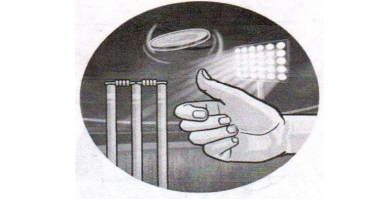
\includegraphics[width=\columnwidth]{./figs/Screenshot (19).png}
        \caption{Tossing a coin}
        \label{fig:2022/probability/fig1.png}
    \end{figure}

Based on the above information, answer the following questions :
\begin{enumerate}[label=(\alph*)]
 \item  If such a coin is tossed $2$ times, then find the probability 
distribution of number of tails.
 
 \item Find the probability of getting at least one head in three tosses of 
such a coin. 
\end{enumerate}

\item Two cards are drawn successively with replacement from a well shuffled pack of $52$ cards. Find the probability distribution of the number of spade cards.

\item A pair of dice is thrown and the sum of the numbers appearing on the dice is observed to be $7$. Find the probability that the number $5$ has appeared on atleast one die.

\item In \figref{fig:2022/probability/fig2.png}, A shopkeeper sells three types of flower seeds $A1$, $A2$, $A3$. They are sold in the form of a mixture, where the proportions of these seeds are $4:4:2$, respectively. The germination rates of the three types of seeds are $45\%$, $60\%$ and $35\%$ respectively.

\begin{figure}[H]
        \centering
        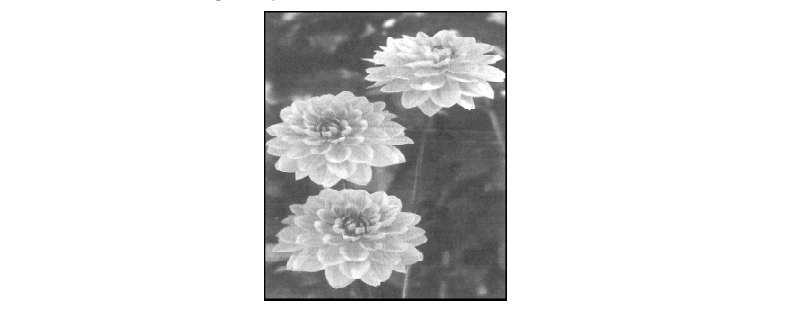
\includegraphics[width=\columnwidth]{./figs/Screenshot (23).png}
        \caption{Three Types of Flower Seeds}
        \label{fig:2022/probability/fig2.png}
    \end{figure}

    Based on the above information:
    
    \begin{enumerate}[label=(\alph*)]
    
 \item Calculate the probability that a randomly chosen seed will germinate;
 
 \item Calculate the probability that the seed is of type $A2$, given that a randomly chosen seed germinates.

\end{enumerate}

\item Three friends $A$, $B$ and $C$ got their photograph clicked. Find the 
probability that $B$ is standing at the central position, given that $A$ is 
standing at the left corner. 

\item In \figref{fig:2022/probability/fig3.png} A coin is tossed twice. The following table shows the probability 
distribution of number of tails :
\begin{figure}[H]
        \centering
        
\includegraphics[width=\columnwidth]{./figs/Screenshot (28).png}
        \caption{Probability Distribution of number of tails}
        \label{fig:2022/probability/fig3.png}
    \end{figure}

    \begin{enumerate}[label=(\alph*)]
    
 \item  Find the value of $K$. 
 
 \item  Is the coin tossed biased or unbiased ? Justify your answer.

\end{enumerate}

\item In \figref{fig:2022/probability/fig4.png} In a game of Archery, each ring of the Archery target is valued. The 
centre most ring is worth $10$ points and rest of the rings are allotted 
points $9$ to $1$ in sequential order moving outwards.

Archer A is likely to earn $10$ points with a probability of $0·8$ and Archer $B$ 
is likely the earn $10$ points with a probability of $0·9$.

\begin{figure}[H]
        \centering
        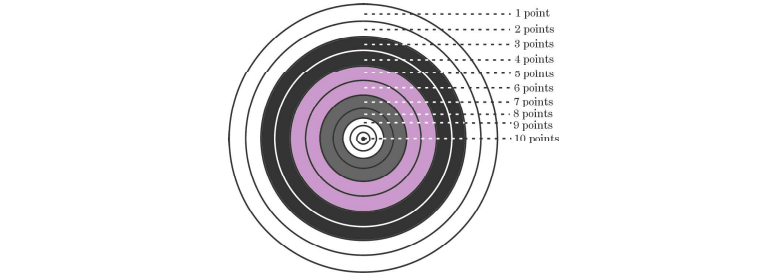
\includegraphics[width=\columnwidth]{./figs/Screenshot (26).png}
        \caption{Ring of the Archery Target}
        \label{fig:2022/probability/fig4.png}
    \end{figure}

Based on the above information, answer the following questions : 
If both of them hit the Archery target, then find the probability that 

\begin{enumerate}[label=(\alph*)]
    
 \item  exactly one of them earns $10$ points.
 
 \item  both of them earn $10$ points.

\end{enumerate}


\item 
\begin{enumerate}[label=(\alph*)]
    
 \item  Events $A$ and $B$ are such that
 P(A) =  $\frac{1}{2}$ , P(B) =  $\frac{7}{12}$  and $ P( \overline{A}  \cup  \overline{B} )= \frac{1}{4}$ Find whether the events $A$ and $B$ are independent or not.
 
 \item  A box $B_{1}$ contains $1$ white ball and $3$ red balls.Another box $B_{2}$ contains $2$ white balls and $3$ red balls.If one ball is drawn at random from each of the boxes $B_{1}$ and $B_{2}$ then find the probability that the two balls drawn are of the same colour.
 
\end{enumerate}

 \item There are two boxes, namely box-I and box-II. Box-I contains $3$ red and $6$ black balls. Box-II contains $5$ red and $5$ black balls. One of the two boxes, is selected at random and a ball is drawn at random. The ball drawn is found to be red. Find the probability that this red ball comes out from box-II.

\item In a toss of three different coins, find the probability of coming up of three heads, if it is known that at least one head comes up.

\item Two rotten apples are mixed with $8$ fresh apples. Find the probability distribution of number of rotten apples, if two apples are drawn at random, one-by-one without replacement.

\item A laboratory blood test is $98\%$ effective in detecting a certain 
disease when it is in fact, present. However, the test also yields 
a false positive result for $0·4\%$ of the healthy person tested. 
From a large population, it is given that 0·2$\%$ of the population 
actually has the disease. 
Based on the above, answer the following questions : 

  \begin{enumerate}[label=(\alph*)]
    
 \item One person, from the population, is taken at random and 
given the test. Find the probability of his getting a 
positive test result.  
 
 \item  What is the probability that the person actually has the 
disease, given that his test result is positive ?

\end{enumerate}

\item Two cards are drawn from a well-shuffled pack of playing 
cards one-by-one with replacement. The probability that the 
first card is a king and the second card is a queen is 

\begin{enumerate}[label=(\alph*)]
    
 \item $\frac{1}{13} + \frac{1}{13}$
 
 \item $\frac{1}{13} \times \frac{4}{51}$

 \item $\frac{4}{52} \times \frac{3}{51}$
 
 \item $\frac{1}{13} \times \frac{1}{13}$ 

\end{enumerate}

\item In \figref{fig:2022/probability/fig5.png} If $X$ is a random variable with probability distribution as given 
below :
\begin{figure}[H]
        \centering
        
\includegraphics[width=\columnwidth]{./figs/Screenshot (32).png}
        \caption{Probability Distribution}
        \label{fig:2022/probability/fig5.png}
    \end{figure}

The value of $k$ and the mean of the distribution respectively 
are

 \begin{enumerate}[label=(\alph*)]
    
 \item  $\frac{1}{7}$,1 
 
 \item  $\frac{1}{6}$,2

 \item  $\frac{1}{6}$,1

 \item  $\frac{1}{6}$

\end{enumerate}


\item For two events $A$ and $B$ if P(A) = $\frac{4}{10}$, P(B) = $\frac{8}{10}$ and 
$ P(B \mid A)$=$\frac{6}{10}$, then find $ P(A \cup B)$.

\item Bag I contains $4$ red and $3$ black balls. Bag II contains $3$ red 
and $5$ black balls. One of the two bags is selected at random 
and a ball is drawn from the bag, which is found to be red. 
Find the probability that the ball is drawn from Bag II.

\item Two cards are drawn successively without replacement from a 
well-shuffled pack of $52$ cards. Find the probability 
distribution of the number of aces and hence find its mean.
\newpage

\item The probability of solving a specific question independently by $A$ and $B$ 
are $\frac{1}{3}$ and $\frac{1}{5}$ respectively. If both try to solve the question independently, 
the probability that the question is solved is 

\begin{enumerate}[label=(\alph*)]
    
 \item  $\frac{7}{15}$
 
 \item  $\frac{8}{15}$
 
 \item  $\frac{2}{15}$
 
 \item  $\frac{14}{15}$

\end{enumerate}

\item A card is picked at random from a pack of $52$ playing cards. Given that 
the picked up card is a queen, the probability of it being a queen of 
spades is ?

\item A bag contains $19$ tickets, numbered $1$ to $19$. A ticket is drawn at random 
and then another ticket is drawn without replacing the first one in the 
bag. Find the probability distribution of the number of even numbers on 
the ticket.

\item Find the probability distribution of the number of successes in two tosses 
of a die, when a success is defined as ‘‘number greater than $5$’’.

\item The random variable $X$ has a probability function $P(x)$ as defined below, 
where $k$ is some number :

\begin{align}
    p(x) = \begin{cases}
        k, & \text{if } x = 0, \\
        2k, & \text{if } x = 1, \\
        3k, & \text{if } x = 2, \\
        0, & \text{otherwise.}
    \end{cases}
\end{align}

Find :
\begin{enumerate}[label=(\roman*)]
 \item The value of $k$
 
 \item $P(X < 2)$, $P(X \leq 2)$, $P(X\ \geq 2)$
 
 \end{enumerate}

\item Consider the following hypothesis :

\begin {align}
H0 : \mu =  35\\
H1 : \mu \neq 35
\end{align}
A sample of $81$ items is taken whose mean is $37·5$ and the standard deviation is $5$. Test the hypothesis at $5\%$ level of significance.

[Given : Critical value of $Z$ for a two-tailed test at $5\%$ level of significance is $1.96$]

\item In \figref{fig:2022/probability/fig6.png} Fit a straight line trend by the method of least squares and find the trend 
value for the year $2008$ for the following data :

\begin{figure}[H]
        \centering
        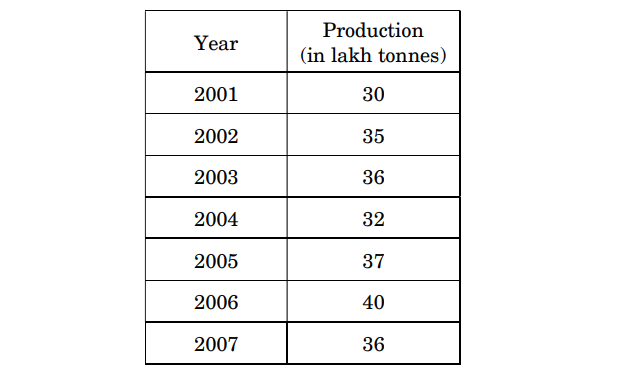
\includegraphics[width=\columnwidth]{./figs/Screenshot (37).png}
        \caption{Years and Production}
        \label{fig:2022/probability/fig6.png}
    \end{figure}
\end{enumerate}

\chapter{Construction}
%\subsection{9}
%\documentclass{article}
%\usepackage{amsmath}
%\usepackage{amssymb}
%\usepackage{amsfonts}
%\usepackage{titling}
%\usepackage{graphicx}

%\providecommand{\abs}[1]{\left\vert#1\right\vert}
%\let\vec\mathbf

%\begin{document}

%\title{\textbf{CONSTRUCTION}}
%\date{}
%\maketitle
\begin{enumerate}


  \item In the given figure, $XZ$ is parallel to $BC$. $AZ$ = 3cm, $ZC$ = 2cm, $BM$ = 3cm and $MC$ = 5cm. Find the length of $XY$.
    \begin{figure}[h!]
      \centering
      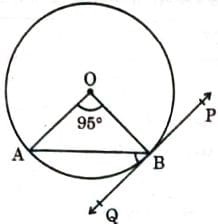
\includegraphics [width=\columnwidth] {figs/fig1.jpg}
      \caption{Isosceles Triangle}
      \label{fig:fig1.jpg}
    \end{figure}

  \item In the given figure, $DE$ $||$ $BC$. If $AD$ = 2units, $DB$ = $AE$ = 3units and $EC$ = $x$units, then find the value of $x$ is:\\

    \begin{figure}[h!]
      \centering
      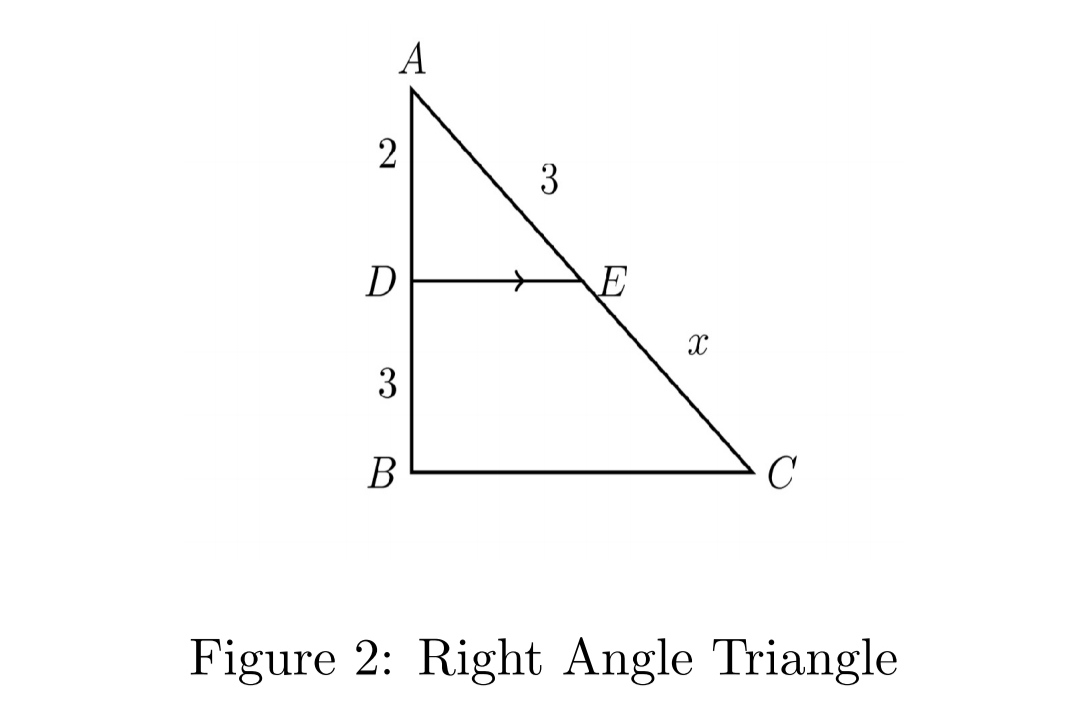
\includegraphics [width=\columnwidth] {figs/fig2.jpg}
      \caption{Right Angle Triangle}
      \label{fig:fig2.jpg}
    \end{figure}

      \begin{enumerate}
        \item 2
        \item 3
        \item 5
        \item $\frac{9}{2}$
      \end{enumerate}

    \newpage

  \item In the given figure, $\Delta ABC$ and $\Delta DBC$ are on te same base $BC$. If $AD$ intersects $BC$ at $\vec{O}$, prove that $\frac { ar(\Delta ABC)}{ar (\Delta DBC)}$ = $\frac{AO}{DO}$.

    \begin{figure}[h!]
      \centering
      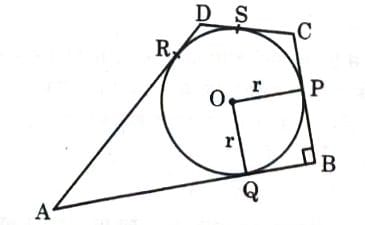
\includegraphics [width=\columnwidth] {figs/fig3.jpg}
      \caption{Triangles with same base}
      \label{fig:fig3.jpg}
    \end{figure}

\end{enumerate}
%\end{document}

\section{2022}
\subsection{10}
\begin{enumerate}[label=\thesection.\arabic*.,ref=\thesection.\theenumi]
\numberwithin{equation}{enumi}
\numberwithin{figure}{enumi}
\numberwithin{table}{enumi}
\item In figure,\figref{fig:rightangled4} BN and CM are medians of a $\triangle$ ABC right-angled at A. Prove that \begin{align}4(BN^2 +CM^2) = 5BC^2\end{align} 
\begin{figure}[!ht]
\centering
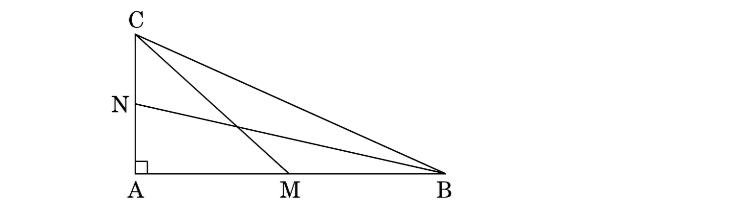
\includegraphics[width=\columnwidth]{figs/rightangled}
\caption{Right-angled triangle}
\label{fig:rightangled4}
\end{figure}
\item $\vec{Case Study - 1:}$
\begin{center}
$\vec{Kite Festival}$\\
\end{center}
Kite festival is celebrated in many countries at different times of the year. in India, every year 14th
January is celebrated as international kite Day. on his day many people visit India and participate in the festival by flying various kinds of kites.
\\The picture given below\figref{fig:kites5} , three kites flying together.
\begin{figure}[!ht]
\centering
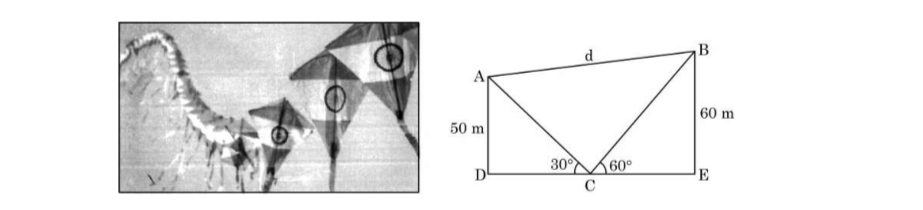
\includegraphics[width=\columnwidth]{figs/kites}
\caption{kites flying to gether}
\label{fig:kites5}
\end{figure}
\\In \figref{fig:kites5}, the angles of elevation of two kites (point C) are found to be $\degree{30}$ and  $\degree{60}$ respectively. Taking \begin{align}AD = 50 m\end{align} and\begin{align} BE = 60 m\end{align}
find 
\begin{enumerate}
\item The length of string used (take them straight) for kites A and B as shown in the figure.
\item The distance 'd' between these two kites
\end{enumerate}
\end{enumerate}
	

\section{2021}
\subsection{10}
%\documentclass{article}
%\usepackage{amsmath} 
%\let\vec\mathbf
%\usepackage{gensymb}
%\usepackage{textcomp}
%\usepackage{enumitem}
%\begin{document}
%\section*{\centering Construction}
\begin{enumerate}[label=\thesection.\arabic*.,ref=\thesection.\theenumi]
\numberwithin{equation}{enumi}
\numberwithin{figure}{enumi}
\numberwithin{table}{enumi}
\item Check whether $13$ cm, $12$ cm, $5$ cm can be the sides of a right triangle.
\item \begin{enumerate}
    \item If a $PL$ and $PM$ are two tangents to a circle with center $\vec{O}$ from an external point $\vec{P}$ and $PL=4$ cm, find the length of $OP$, where radius of the circle is $3$ cm.
    \item Find the distance between two parallel tangents of a circle of radius $2.5$ cm.
\end{enumerate}
    \item 
    \begin{enumerate}
    \item $\vec{D}$ and $\vec{E}$ are points on the sides $CA$ and $CB$ respectively of  a triangle $ABC$, right-angled at $\vec{C}$.
    
    Prove that $AE^2+BD^2=AB^2+DE^2$.
    
    \item Diagonals of a trapezium $ABCD$ with $AB\parallel DC$ intersect each other at the point $\vec{O}$. If $AB=2CD$, find the ratio of the areas of triangles $AOB$ and $COD$.
    \end{enumerate}

    \item Answer any \textbf{four} of the following questions :
      \begin{enumerate}[label=(\roman*)]
        \item Given $\triangle ABC \sim \triangle PQR$. If $\frac{AB}{PQ}=\frac{1}{3}$,then $\frac{ar(\triangle ABC)}{ar(\triangle PQR)}$ is 
        \begin{enumerate}[label=(\Alph*)]
            \item $\frac{1}{3}$
            \item $3$
            \item $\frac{2}{3}$
            \item $\frac{1}{9}$
        \end{enumerate}
        
        \item The length of an altitude of an equilateral triangle of side $8$ cm is
        
          \begin{enumerate}[label=(\Alph*)]
            \item $4$ cm
            \item $4\sqrt{3}$ cm
            \item $\frac{8}{3}$ cm
            \item $12$ cm
        \end{enumerate}
        
        \item In $\triangle PQR$, $PQ=6\sqrt{3}$ cm, $PR=12 cm$ and $QR = 6$ cm. The measure of angle $\vec{Q}$ is
        
        \begin{enumerate}[label=(\Alph*)]
            \item $120\degree$
            \item $60\degree$
            \item $90\degree$
            \item $40\degree$
        \end{enumerate}
        
        \item If $\triangle ABC\sim\triangle PQR$ and $\angle B=46\degree$ and $\angle R=69\degree$, then the measure of $\angle$A is
        \begin{enumerate}[label=(\Alph*)]
            \item $65\degree$
            \item $111\degree$
            \item $44\degree$
            \item $115\degree$
        \end{enumerate}
        
        \item $\vec{P}$ and $\vec{Q}$ are the points on the sides $AB$ and $AC$ respectively of a $\triangle ABC$ such that $PQ\parallel BC$. If $AP:PB=2:3$ and $AQ=4$ cm,then $AC$ is equal to

        \begin{enumerate}[label=(\Alph*)]
            \item $6$ cm
            \item $8$ cm
            \item $10$ cm
            \item $12$ cm
        \end{enumerate}
        \end{enumerate}
        \item Write the steps of construction of drawing a line segment $AB=4.8$ cm and finding a point $\vec{P}$ on it such that $AP=\frac{1}{4}AB$.
        
        \item Answer any \textbf{four} of the following questions :
        \begin{enumerate}[label=(\roman*)]
        \item $ABC$ and $BDE$ are two equilateral triangles such that $\vec{D}$ is the mid-point of $BC$. The ratio of the areas of the triangles $ABC$ and $BDE$ is
        \begin{enumerate}[label=(\Alph*)]
            \item 2:1
            \item 1:2
            \item 4:1
            \item 1:4
        \end{enumerate}
        
        \item In $\triangle$ ABC , $AB=4\sqrt{3}$ cm, $AC=8$ cm and $BC=4$ cm. The angle $B$ is

        \begin{enumerate}[label=(\Alph*)]
            \item $120\degree$
            \item $90\degree$
            \item $60\degree$
            \item $45\degree$
        \end{enumerate}
         
        \item The perimeters of two similar triangles are $35$ cm and $21$ cm respectively.  If one side of the first triangle is $9$ cm, then the corresponding side of the second triangle is 
        
         \begin{enumerate}[label=(\Alph*)]
            \item $5.4$ cm
            \item $4.5$ cm
            \item $5.6$ cm
            \item $15$ cm
        \end{enumerate}
        
        \item In a $\triangle ABC$ , $\vec{D}$ and $\vec{E}$ are points on the sides $AB$ and $AC$ respectively such that $DE\parallel BC$ and $AD:DB=3:1$. If $AE=3.3 $ cm, then $AC$ is equal to
        \begin{enumerate}[label=(\Alph*)]
            \item $4$ cm
            \item $1.1$ cm
            \item $4.5$ cm
            \item $5.5$ cm
        \end{enumerate}
        
        \item In an isosceles triangle $ABC$, if $AC=BC$ and $AB^2=2AC^2$, the $\angle$C is equal to
        \begin{enumerate}[label=(\Alph*)]
            \item $30\degree$
            \item $45\degree$
            \item $60\degree$
            \item $90\degree$
        \end{enumerate}
        \end{enumerate}
\end{enumerate}
%\end{document}


\chapter{Optimization}
\section{2023}

\begin{enumerate}
	\item The objective function $Z = ax+by$ of an LLP has maximum value 42 at (4,6) and minimum value 19 at (3,2).Which of the following is true?
		
  		\begin{enumerate}
				\item $a=9,b=1$
		        	\item $a=5,b=2$
				\item $a= 3,b=5$
				\item $a=5,b=3$
			
		\end{enumerate}
		
	\item The corner point of the feasible region of a linear programming problem are (0,4), (8,0)and ($\frac{20}{3}$,$\frac{4}{3}$).if $ Z=30x+24y $ is the objective fnction, then ( maximum value of Z-minimum value of Z) is equal to 
		
		\begin{enumerate}
				\item 40
				\item 96
				\item 120
				\item 136
		\end{enumerate}
		
		
	\item 
	 Solve the following linear programming problem graphically :
\begin{align}
	Maximum:& Z=x+2y \nonumber \\
	subject to constraints 
	     :& x+2y\ge100 ,\nonumber\\
             &  2x-y\le0 ,\nonumber\\
	     &  2x+y\le200 ,\nonumber\\
   	     &   x\ge0 ,y\ge0 .\nonumber
\end{align}
				

			      \item
		Engine displacement is the measure of the cylinder volume swept by all the pistons engine.The piston move inside the cylinder bore \\
		
		\begin{figure}[htbp]
	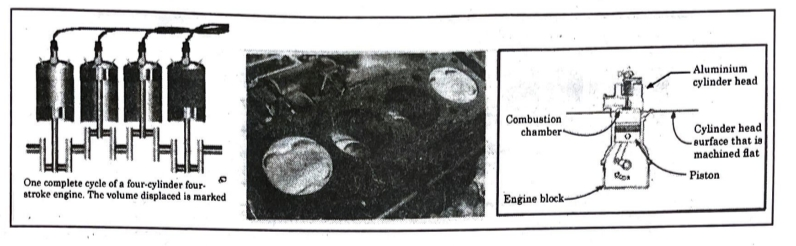
\includegraphics[width=1 \columnwidth]{./figs/engine.jpg}\\
			\caption{Engine}
			\label{fig:pic}  \end{figure}
		The cylinder bore in the form of circular cylinder open at the top is to be made from a metal sheet of area $ 75 \pi cm^2 $ \\
 	
		Based on the above information,answer the following questions:\\
		
			\begin{enumerate}
				\item if the radius of cylinder is r cm and height is h cm,then write the volme V of cylinder in terms of radius r.
					
				\item Find $ \frac{dV}{dr} $.
					
				\item \begin{enumerate}
						\item Find the radius of cylinder when its volume is maximum.
			
		\item For maximum volume,$h>r$.State true or false and justify.
				
			
				\end{enumerate}
			\end{enumerate}
\end{enumerate}

\section{2021}
\subsection{12}
\begin{enumerate}
  
\item A company produces two types of goods, $A$ and $B$, that require gold and
silver. Each unit of type $A$ requires $3g$ of silver and $1g$ of gold, while that of type $B$ requires $1g$ of silver and $2g$ of gold. The company can use at
the most $9g$ of silver and $8g$ of gold. If each unit of type $A$ brings a profit
of \rupee~120 and that of type $B$ \rupee~150, then find the number of units of each type that the company should produce to maximise profit. Formulate the above LPP and solve it graphically. Also, find the maximum profit.
\item Find the maximum value of $7x+6y$ subject to the constrains:
\begin{align}
	x+y &\geq   2\\
	2x+3y &\leq 6\\
	x \geq 0 \text{and} y &\geq 0
\end{align}
\item A window is in the form of a rectangular mounted by a semi-circular opening.The total perimeter of the window to admit maximum light through the whole opening.
\item Divide the number $8$ into two positive numbers such that the sum of the cube of one and the square of the other is maximum.
\item Find the maximum and the minimum values of 
\begin{align}
       z=5x+2y 
\end{align}	
		subject to the constrains:
\begin{align}
	-2x-3y &\leq -6\\
	x-2y &\leq 2\\
	6x+4y &\leq 24\\
	-3x+2y &\leq 3\\
	x \geq 0, y &\geq 0
\end{align}
 
 \item A furniture dealer deals in only two items : chairs and tables. He has \rupee~5,000  to invest and a space to store at most $60$ pieces. A table costs him \rupee~250 and a chair \rupee~50. He sells a table at a profit of \rupee~50 and a chair at
a profit of \rupee~ 15. Assuming that he can sell all the items he buys, how should he invest his money in order that he may maximize his profit ?
Formulate the above as a linear programming problem.
\item The least value of the function 
\begin{align}
	f(x)=2\cos(x) + x
\end{align}
		in the closed interval $\sbrak{0, \frac{\pi}{2}}$ is: 
\begin{enumerate}
    \item  $2$
    \item  $\frac{\pi}{6} + \sqrt{3}$
    \item  $\frac{\pi}{2}$
    \item The least value does not exist.
\end{enumerate}
\item A linear programming problem is as follows:
Minimize 
\begin{align}
	Z=30x+50y 
\end{align}
		subject to the constrains,
\begin{align}
	3x+5y &\geq 15\\
	2x+3y &\leq 18\\
	x \geq 0, y &\geq 0
\end{align}
In the feasible region, the minimum value of $Z$ occurs at 
\begin{enumerate}
    \item a unique point 
    \item no point
    \item infinitely many points 
    \item two points only
\end{enumerate}
\item The area of a trapezium is defined by function $f$
and given by 
\begin{align}
	f(x)=(10+x)\sqrt{100-x^2}
\end{align}
			, then the area when it is maximised is:
\begin{enumerate}
    \item $75cm^2$
    \item $7\sqrt{3}cm^2$
    \item $75\sqrt{3}cm^2$
    \item $5cm^2$
\end{enumerate}
\item For an objective function 
\begin{align}
	Z=ax+by
\end{align}		
		,where $a,b>0$;the corner points of the feasible region determined by a set of constrains (linear inequalities) are $(0,20)$, $(10,10)$, $(30,30)$, and $(0,40)$.The condition on $a$ and $b$ such that the maximum $Z$ occurs at the points $(30,30)$ and $(0,40)$ is: 
\begin{enumerate}
    \item $b-3a=0$
    \item $a=3b$
    \item $a+2b=0$
    \item $2a-b=0$
\end{enumerate}
\item In a linear programming problem, the constrains on the decision variables $x$ and $y$ are $x-3y \geq 0, y \geq 0, 0\leq x \leq 3$.The feasible region 
\begin{enumerate}
    \item is not in the first quadrant
    \item is bounded in the first quadrant 
    \item is unbounded in the first quadrant 
    \item does not exist  
\end{enumerate}
\item Based on the given shaded region in figure \ref{fig:19/2021/041} as the feasible region in the graph, at which point(S) is the objective function 
\begin{align}
	Z=3x+9y 
\end{align}
		maximum?
\begin{figure}[h]
    \centering{}
    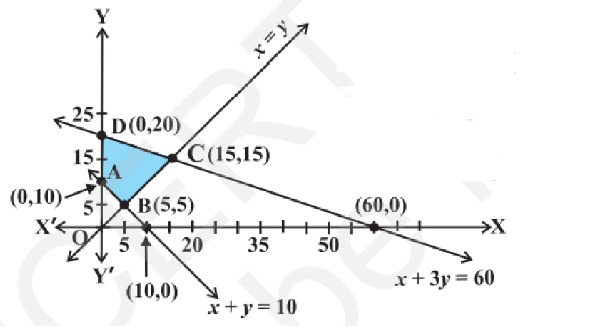
\includegraphics[width=\columnwidth]{figs/opti-21-fig1.jpg}
	\caption{Optimization graph}
    \label{fig:19/2021/041}
\end{figure}
\begin{enumerate}
    \item point $B$
    \item point $C$
    \item point $D$
    \item every point on the line segment $CD$   
\end{enumerate}
\item In figure \ref{fig:23/2021/041}, the feasible region for a LPP is shaded.The objective function 
\begin{align}
	Z=2x-3y
\end{align}
		,will be minimum at:
\begin{figure}[h]
    \centering{}
     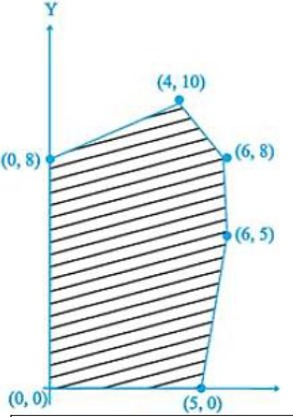
\includegraphics[width=\columnwidth]{figs/opti-21-fig2.jpg}
	\caption{Optimization graph}
     \label{fig:23/2021/041}                       
\end{figure}
\begin{enumerate}
    \item $(4,10)$
    \item $(6,8)$
    \item $(0,8)$
    \item $(6,5)$
\end{enumerate}
    
\end{enumerate}

\chapter{Algebra}
\section{2023}
\subsection{10}
%\documentclass{article}
%\begin{document}
\begin{enumerate}
 \item If one zero of the polynomial \begin{align} p(x)=6x^2+37x-(k-2) \end{align} is reciprocal of the other, then find the value of $k$?
 \item Find the value of $'p'$ for which one root of the quadratic equation \begin{align} px^2-14x+18=0 \end{align}is 6 times the other?
 \item 
 \begin{enumerate}
  \item prove that \begin{align} \frac{\sin A-2 \sin^3A}{2\cos^3A-\cos A}=\tan A\end{align} 
  \item \begin{align} \sec A (1-\sin A)(\sec A+\tan A)=1\end{align} 
  \end{enumerate}
  \item Which of the following  quadratic equations has sum of its roots as 4?
  \begin{enumerate}
      \item $2x^2-4x+8=0$ 
      \item $-x^2+4x+4=0$
      \item $\sqrt{2x^2}-\frac{4}{\sqrt{2}}x+1=0$ 
      \item $4x^2-4x+4=0$
   \end{enumerate}
   \item if one zero of the polynomial \begin{align} 6x^2+37x-(k-2)\end{align}  is reciprocal of the other,then what is the value of $k$?
   \begin{enumerate}
       \item -4
       \item -6
       \item 6
       \item 4
   \end{enumerate}
   \item The zeroes of the polynomial \begin{align}p(x)=x^2+4x+3\end{align}  are given by:
   \begin{enumerate}
       \item 1,3
       \item -1,3
       \item 1,-3
       \item -1,-3
   \end{enumerate}
\item If $\alpha$ and $\beta$ are the zeroes of the quadratic polynomial $p(x)=x^2-ax-b$, then the value of $\alpha^2 + \beta^2$ is:


\begin{enumerate}
\item $a^2-2b$
\item $a^2+2b$
\item $b^2-2a$
\item $b^2+2a$
\end{enumerate}

\item The below is the Assertion and Reason based question. Two statements are given, one labelled as Assertion(A) and the other is labelled as Reason(R). Select the correct answer to these questions from the codes (a),(b),(c) and (d) as given below.
\begin{enumerate}
\item Both Assertion(A) and Reason(R) are true and Reason(R) is the correct explanation of the Assertion(A).
\item Both Assertion(A) and Reason(R) are true, but Reason(R) is not the correct explanation of the Assertion(A).
\item Assertion(A) is true, but Reason(R) is false.
\item Assertion(A) is false, but Reason(R) is true.\\ 
\textbf{Assertion(A):} The polynomial $p(x)=x^2+3x+3$ has two real zeroes.\\
\textbf{Reason(R):} A quadratic polynomial can have at most two real zeroes.

\end{enumerate}

\item
\begin{enumerate}
\item If 
\begin{align}
    4\cot^2 45\degree - \sec^2 60\degree + \sin^2 60\degree + p = \frac{3}{4}, 
\end{align}
then find the value of $p$.
\item If 
\begin{align}
    \cos A+ \cos^2A=1,
\end{align}then find the value of 
\begin{align}
\sin^2A+\sin^4A.
\end{align}
\end{enumerate}


\item Prove that:\\
\begin{align}
\brak{\frac{1}{\cos\theta}-\cos\theta}\brak{\frac{1}{\sin\theta}-\sin\theta} = \frac{1}{\tan\theta+\cot\theta}
\end{align}


\item The value of k for which the pair of equations $kx=y+2$ and $6x=2y+3$ has infinitely many solutions,
\begin{enumerate}
\item is $k=3$
\item does not exist
\item is $k=-3$
\item is $k=4$
\end{enumerate}


\item If $2\tan A=3$, then the value of $\frac{4sin A + 3\cos A}{4\sin A - 3\cos A}$ is
\begin{enumerate}
\item $\frac{7}{\sqrt{13}}$
\item $\frac{1}{\sqrt{13}}$
\item $3$
\item does not exist
\end{enumerate}


\item If $\alpha$, $\beta$ are the zeroes of a polynomial $p(x)=x^2+x-1$, then $\frac{1}{\alpha}+\frac{1}{\beta}$ equals to 
\begin{enumerate}
\item $1$
\item $2$
\item $-1$
\item $\frac{-1}{2}$
\end{enumerate}

    \item $\brak{\sec^2\theta - 1}\brak{\csc^2\theta - 1}$  is equal to:
    \begin{enumerate}
        \item $-1$
        \item  $1$
        \item  $0$
        \item  $2$
        \end{enumerate}
    \item The roots of equation 
    \begin{align}
        x^2 + 3x - 10 = 0
    \end{align}
    are:
    \begin{enumerate}
        \item $\brak{2,-5}$
        \item $\brak{-2,5}$
        \item $\brak{2,5}$
        \item $\brak{-2,-5}$
    \end{enumerate}
    \item If $\alpha$ , $\beta$ are zeroes of the polynomial $x^2-1$,then value of $\brak{\alpha+\beta}$ is:
    \begin{enumerate}
        \item $2$
        \item $1$
        \item $1$
        \item $0$
    \end{enumerate}
    \pagebreak
   \item  If $\alpha$, $\beta$ are the zeroes of the polynomial
   \begin{align}
       p(x)=4x^2 - 3x -7
   \end{align}
   ,then $\brak{\frac{1}{\alpha}+\frac{1}{\beta}}$ is equal to:
   \begin{enumerate}
       \item $\frac{7}{3}$
       \item $\frac{-7}{3}$
       \item $\frac{3}{7}$
       \item $\frac{-3}{7}$
   \end{enumerate}
   \item  Find the sum and product of the roots of the quadratic equation 
   \begin{align}
       2x^2-9x+4=0
   \end{align}
   \item Find the discriminant of the quadratic equation 
   \begin{align}
       4x^2-5=0
   \end{align}
   and hence comment on the nature of roots of the equation.
   \item Evaluate $2\sec^2\theta+3\csc^2\theta-2\sin\theta\cos\theta$ if
   \begin{align}
      \theta=45\degree
   \end{align}
   
   \item If
   \begin{align}
       \sin\theta-\cos\theta=0
   \end{align}
   ,then find the value of $\sin^4\theta+\cos^4\theta$.

\end{enumerate}
%\end{document}

%


%\include{ch02} 
\backmatter
\appendix
\iffalse
\chapter{Conic Lines}
\section{Pair of Straight Lines}
%
\input{quad/pair.tex}
\section{Intersection of Conics}
\input{quadlines/inter.tex}
\section{ Chords of a Conic}
\input{quadlines/chord.tex}
\section{ Tangent and Normal}
\begin{enumerate}
\item Find the equation of tangent to the curve $y = x^2 + 4x + 1$ at the point $(3,22)$.
\end{enumerate}		

\fi
%\chapter{Proofs}
%   \section{}
%\input{apps/defs.tex}

%  \section{}
%\input{apps/parab.tex}
%  \section{}
%\input{apps/nonparab.tex}
%		\section{}
%\input{apps/params.tex}
\latexprintindex

\end{document}

 
\section{Examples}
\subsection{Loney}
\input{examples/loney.tex}
\subsection{Miscellaneous}
%\documentclass{exam}
%\usepackage{float}
%\usepackage{array}
%\usepackage{enumitem}
%\usepackage{amsmath}
%\begin{document}
\begin{enumerate}
	
	\item Find the distance of the point $(1,-2,9)$ from the point of intersection of the line
		\begin{align}
			\vec{r}=4\hat{i}+2\hat{j}+7\hat{k}+\lambda(3\hat{i}+4\hat{j}+2\hat{k})
		\end{align}and the plane
		\begin{align}
			\vec{r}\cdot(\hat{i}-\hat{j}+\hat{k})=10.
		\end{align}

	\item Find the area bounded by the curves $y=\abs{x-1}$ and $y=1$, using integration.

	\item Find the coordinates of the point where the line through $(4,-3,-4)$ and $(3,-2,2)$ crosses the plane $2x+y+z=6$.

	\item Fit a straight line trend by the method of least squares and find the trend value for the year 2008 using the data from Table \ref{tab:LC}:
		\begin{table}[H]
			\caption{Table showing yearly trend of production of goods in lakh tonnes \label{tab:LC}}
			%%%%%%%%%%%%%%%%%%%%%%%%%%%%%%%%%%%%%%%%%%%%%%%%%%%%%%%%%%%%%%%%%%%%%%
%%                                                                  %%
%%  This is the header of a LaTeX2e file exported from Gnumeric.    %%
%%                                                                  %%
%%  This file can be compiled as it stands or included in another   %%
%%  LaTeX document. The table is based on the longtable package so  %%
%%  the longtable options (headers, footers...) can be set in the   %%
%%  preamble section below (see PRAMBLE).                           %%
%%                                                                  %%
%%  To include the file in another, the following two lines must be %%
%%  in the including file:                                          %%
%%        \def\inputGnumericTable{}                                 %%
%%  at the beginning of the file and:                               %%
%%        \input{name-of-this-file.tex}                             %%
%%  where the table is to be placed. Note also that the including   %%
%%  file must use the following packages for the table to be        %%
%%  rendered correctly:                                             %%
%%    \usepackage[latin1]{inputenc}                                 %%
%%    \usepackage{color}                                            %%
%%    \usepackage{array}                                            %%
%%    \usepackage{longtable}                                        %%
%%    \usepackage{calc}                                             %%
%%    \usepackage{multirow}                                         %%
%%    \usepackage{hhline}                                           %%
%%    \usepackage{ifthen}                                           %%
%%  optionally (for landscape tables embedded in another document): %%
%%    \usepackage{lscape}                                           %%
%%                                                                  %%
%%%%%%%%%%%%%%%%%%%%%%%%%%%%%%%%%%%%%%%%%%%%%%%%%%%%%%%%%%%%%%%%%%%%%%



%%  This section checks if we are begin input into another file or  %%
%%  the file will be compiled alone. First use a macro taken from   %%
%%  the TeXbook ex 7.7 (suggestion of Han-Wen Nienhuys).            %%
\def\ifundefined#1{\expandafter\ifx\csname#1\endcsname\relax}


%%  Check for the \def token for inputed files. If it is not        %%
%%  defined, the file will be processed as a standalone and the     %%
%%  preamble will be used.                                          %%
\ifundefined{inputGnumericTable}

%%  We must be able to close or not the document at the end.        %%
 \def\gnumericTableEnd{\end{document}}


%%%%%%%%%%%%%%%%%%%%%%%%%%%%%%%%%%%%%%%%%%%%%%%%%%%%%%%%%%%%%%%%%%%%%%
%%                                                                  %%
%%  This is the PREAMBLE. Change these values to get the right      %%
%%  paper size and other niceties.                                  %%
%%                                                                  %%
%%%%%%%%%%%%%%%%%%%%%%%%%%%%%%%%%%%%%%%%%%%%%%%%%%%%%%%%%%%%%%%%%%%%%%

 \documentclass[12pt%
     %,landscape%
                    ]{report}
       \usepackage[latin1]{inputenc}
       \usepackage{fullpage}
       \usepackage{color}
       \usepackage{array}
       \usepackage{longtable}
       \usepackage{calc}
       \usepackage{multirow}
       \usepackage{hhline}
       \usepackage{ifthen}

 \begin{document}


%%  End of the preamble for the standalone. The next section is for %%
%%  documents which are included into other LaTeX2e files.          %%
\else

%%  We are not a stand alone document. For a regular table, we will %%
%%  have no preamble and only define the closing to mean nothing.   %%
    \def\gnumericTableEnd{}

%%  If we want landscape mode in an embedded document, comment out  %%
%%  the line above and uncomment the two below. The table will      %%
%%  begin on a new page and run in landscape mode.                  %%
%       \def\gnumericTableEnd{\end{landscape}}
%       \begin{landscape}


%%  End of theelse clause for this file being \input.              %%
\fi

%%%%%%%%%%%%%%%%%%%%%%%%%%%%%%%%%%%%%%%%%%%%%%%%%%%%%%%%%%%%%%%%%%%%%%
%%                                                                  %%
%%  The rest is the gnumeric table, except for the closing          %%
%%  statement. Changes below will alter the table's appearance.     %%
%%                                                                  %%
%%%%%%%%%%%%%%%%%%%%%%%%%%%%%%%%%%%%%%%%%%%%%%%%%%%%%%%%%%%%%%%%%%%%%%

\providecommand{\gnumericmathit}[1]{#1} 
%%  Uncomment the next line if you would like your numbers to be in %%
%%  italics if they are italizised in the gnumeric table.           %%
%\renewcommand{\gnumericmathit}[1]{\mathit{#1}}
\providecommand{\gnumericPB}[1]%
{\let\gnumericTemp=\\#1\let\\=\gnumericTemp\hspace{0pt}}
 \ifundefined{gnumericTableWidthDefined}
        \newlength{\gnumericTableWidth}
        \newlength{\gnumericTableWidthComplete}
        \newlength{\gnumericMultiRowLength}
        \global\def\gnumericTableWidthDefined{}
 \fi
%% The following setting protects this code from babel shorthands.  %%
 \ifthenelse{\isundefined{\languageshorthands}}{}{\languageshorthands{english}}
%%  The default table format retains the relative column widths of  %%
%%  gnumeric. They can easily be changed to c, r or l. In that case %%
%%  you may want to comment out the next line and uncomment the one %%
%%  thereafter                                                      %%
\providecommand\gnumbox{\makebox[0pt]}
%%\providecommand\gnumbox[1][]{\makebox}

%% to adjust positions in multirow situations                       %%
\setlength{\bigstrutjot}{\jot}
\setlength{\extrarowheight}{\doublerulesep}

%%  The \setlongtables command keeps column widths the same across  %%
%%  pages. Simply comment out next line for varying column widths.  %%
\setlongtables

\setlength\gnumericTableWidth{%
 53pt+%
 53pt+%
 106pt+%
0pt}
\def\gumericNumCols{3}
\setlength\gnumericTableWidthComplete{\gnumericTableWidth+%
         \tabcolsep*\gumericNumCols*2+\arrayrulewidth*\gumericNumCols}
\ifthenelse{\lengthtest{\gnumericTableWidthComplete > \linewidth}}%
         {\def\gnumericScale{\ratio{\linewidth-%
                        \tabcolsep*\gumericNumCols*2-%
                        \arrayrulewidth*\gumericNumCols}%
{\gnumericTableWidth}}}%
{\def\gnumericScale{1}}

%%%%%%%%%%%%%%%%%%%%%%%%%%%%%%%%%%%%%%%%%%%%%%%%%%%%%%%%%%%%%%%%%%%%%%
%%                                                                  %%
%% The following are the widths of the various columns. We are      %%
%% defining them here because then they are easier to change.       %%
%% Depending on the cell formats we may use them more than once.    %%
%%                                                                  %%
%%%%%%%%%%%%%%%%%%%%%%%%%%%%%%%%%%%%%%%%%%%%%%%%%%%%%%%%%%%%%%%%%%%%%%

\ifthenelse{\isundefined{\gnumericColA}}{\newlength{\gnumericColA}}{}\settowidth{\gnumericColA}{\begin{tabular}{@{}p{53pt*\gnumericScale}@{}}x\end{tabular}}
\ifthenelse{\isundefined{\gnumericColB}}{\newlength{\gnumericColB}}{}\settowidth{\gnumericColB}{\begin{tabular}{@{}p{150pt*\gnumericScale}@{}}x\end{tabular}}
\ifthenelse{\isundefined{\gnumericColC}}{\newlength{\gnumericColC}}{}\settowidth{\gnumericColC}{\begin{tabular}{@{}p{106pt*\gnumericScale}@{}}x\end{tabular}}

\begin{longtable}[c]{%
 b{\gnumericColA}%
 b{\gnumericColB}%
 b{\gnumericColC}%
 }

%%%%%%%%%%%%%%%%%%%%%%%%%%%%%%%%%%%%%%%%%%%%%%%%%%%%%%%%%%%%%%%%%%%%%%
%%  The longtable options. (Caption, headers... see Goosens, p.124) %%
% \caption{The Table Caption.}             \\ %
% \hline % Across the top of the table.
%%  The rest of these options are table rows which are placed on    %%
%%  the first, last or every page. Use \multicolumn if you want.    %%

%%  Header for the first page.                                      %%
% \multicolumn{3}{c}{The First Header} \\ \hline 
% \multicolumn{1}{c}{colTag} %Column 1
% &\multicolumn{1}{c}{colTag} %Column 2
% &\multicolumn{1}{c}{colTag} \\ \hline %Last column
% \endfirsthead

%%  The running header deinition.

%%
% \hline
% \multicolumn{3}{l}{\ldots\small\slshape continued} \\ \hline
% \multicolumn{1}{c}{colTag} %Column 1
% &\multicolumn{1}{c}{colTag} %Column 2
% &\multicolumn{1}{c}{colTag} \\ \hline %Last column
% \endhead

%%  The running footer definition.                                  %%
% \hline
% \multicolumn{3}{r}{\small\slshape continued\ldots} \\
% \endfoot

%%  The ending footer definition.                                   %%
% \multicolumn{3}{c}{That's all folks} \\ \hline 
% \endlastfoot
%%%%%%%%%%%%%%%%%%%%%%%%%%%%%%%%%%%%%%%%%%%%%%%%%%%%%%%%%%%%%%%%%%%%%%

\hhline{|-|-|-}
  \multicolumn{1}{|p{\gnumericColA}|}%
 {\gnumericPB{\raggedright}\gnumbox[l]{Year}}
 &\multicolumn{1}{p{\gnumericColB}|}%
	{\gnumericPB{\raggedright}\gnumbox[l]{Production (in lakh tonnes)}}
 %&\multicolumn{1}{p{\gnumericColC}|}%
 %{\gnumericPB{\raggedright}\gnumbox[l]{Description}}
\\
\hhline{|---|}
  \multicolumn{1}{|p{\gnumericColA}|}%
 {\gnumericPB{\raggedright}\gnumbox[l]{2001}}
 &\multicolumn{1}{p{\gnumericColB}|}%
 {\gnumericPB{\raggedright}\gnumbox[l]{30}}
 %&\multicolumn{1}{p{\gnumericColC}|}%
 %{\gnumericPB{\raggedright}\gnumbox[l]{Vertex A}}
\\
\hhline{|---|}
  \multicolumn{1}{|p{\gnumericColA}|}%
 {\gnumericPB{\raggedright}\gnumbox[l]{2002}}
 &\multicolumn{1}{p{\gnumericColB}|}%
 {\gnumericPB{\raggedright}\gnumbox[l]{35}}
 %&\multicolumn{1}{p{\gnumericColC}|}%
 %{\gnumericPB{\raggedright}\gnumbox[l]{Vertex B}}
\\
\hhline{|---|}
  \multicolumn{1}{|p{\gnumericColA}|}%
 {\gnumericPB{\raggedright}\gnumbox[l]{2003}}
 &\multicolumn{1}{p{\gnumericColB}|}%
 {\gnumericPB{\raggedright}\gnumbox[l]{36}}
 %&\multicolumn{1}{p{\gnumericColC}|}%
 %{\gnumericPB{\raggedright}\gnumbox[l]{Vertex C}}
\\
\hhline{|---|}
  \multicolumn{1}{|p{\gnumericColA}|}%
 {\gnumericPB{\raggedright}\gnumbox[l]{2004}}
 &\multicolumn{1}{p{\gnumericColB}|}%
 {\gnumericPB{\raggedright}\gnumbox[l]{32}}
 %&\multicolumn{1}{p{\gnumericColC}|}%
 %{\gnumericPB{\raggedright}\gnumbox[l]{Midpoint of AC}}
\\
\hhline{|---|}
  \multicolumn{1}{|p{\gnumericColA}|}%
 {\gnumericPB{\raggedright}\gnumbox[l]{2005}}
 &\multicolumn{1}{p{\gnumericColB}|}%
 {\gnumericPB{\raggedright}\gnumbox[l]{37}}
 %&\multicolumn{1}{p{\gnumericColC}|}%
 %{\gnumericPB{\raggedright}\gnumbox[l]{Midpoint of BC}}
\\
\hhline{|---|}
  \multicolumn{1}{|p{\gnumericColA}|}%
 {\gnumericPB{\raggedright}\gnumbox[l]{2006}}
 &\multicolumn{1}{p{\gnumericColB}|}%
 {\gnumericPB{\raggedright}\gnumbox[l]{40}}
 %&\multicolumn{1}{p{\gnumericColC}|}%
 %{\gnumericPB{\raggedright}\gnumbox[l]{Midpoint of AB}}
\\
\hhline{|-|-|-|}
\end{longtable}

\ifthenelse{\isundefined{\languageshorthands}}{}{\languageshorthands{\languagename}}
\gnumericTableEnd

		\end{table}
\end{enumerate}
%\end{document}

%
%%\section*{Disclosure Statement}
%%The authors report there are no competing interests to declare.
%%
%%
%%
%%  
%%%All the results related to conics are summarized in 
%%%Table \ref{table:conics}.  
%%%\begin{table*}[!t]
%%%\centering
%%%\input{conics.tex}
%%%%\input{./figs/conics.tex}
%%%\caption{$\vec{x}^{\top}\vec{V}\vec{x}+2\vec{u}^{\top}\vec{x}+f = 0$  can be expressed in the above standard form for various conics. $\vec{c}$ represents the centre/vertex of the conic. $\vec{q}$ is/are the point(s) of contact for the tangent(s). }
%%%\label{table:conics}
%%%\end{table*}
%%%\begin{verbatim}
%%\bibliographystyle{tfs}
%%%\bibliography{interacttfssample}
%%\bibliography{school}
%%\end{verbatim}
%% included where the list of references is to appear, where \texttt{tfs.bst} is the name of the \textsc{Bib}\TeX\ bibliography style file for Taylor \& Francis' Reference Style S and \texttt{interacttfssample.bib} is the bibliographic database included with the \textsf{Interact}-TFS \LaTeX\ bundle (to be replaced with the name of your own .bib file). \LaTeX/\textsc{Bib}\TeX\ will extract from your .bib file only those references that are cited in your .tex file and list them in the References section.
%
%% Please include a copy of your .bib file and/or the final generated .bbl file among your source files if your .tex file does not contain a reference list in a \texttt{thebibliography} environment.
%

  % \section{Appendices}
  % \appendix
			\appendices
